\documentclass{beamer}

\mode<presentation>
{
  \usetheme{Goettingen}
  \usecolortheme{seahorse}
  \setbeamercovered{transparent}
}

\usepackage[english]{babel}
\usepackage[latin1]{inputenc}

\usepackage{graphicx}
\graphicspath{ {images/} }

\usepackage{times}
\usepackage[T1]{fontenc}

\title{Nets and tilings as models for crystals}

\author[Olaf Delgado]{Olaf Delgado-Friedrichs}

\date{CG Week Brisbane, 4 July 2017}

\begin{document}

\begin{frame}
  \titlepage
\end{frame}

%\begin{frame}{Outline}
%  \tableofcontents
%\end{frame}

\section{Crystal Model Hierarchy}

\begin{frame}
  \begin{center}
    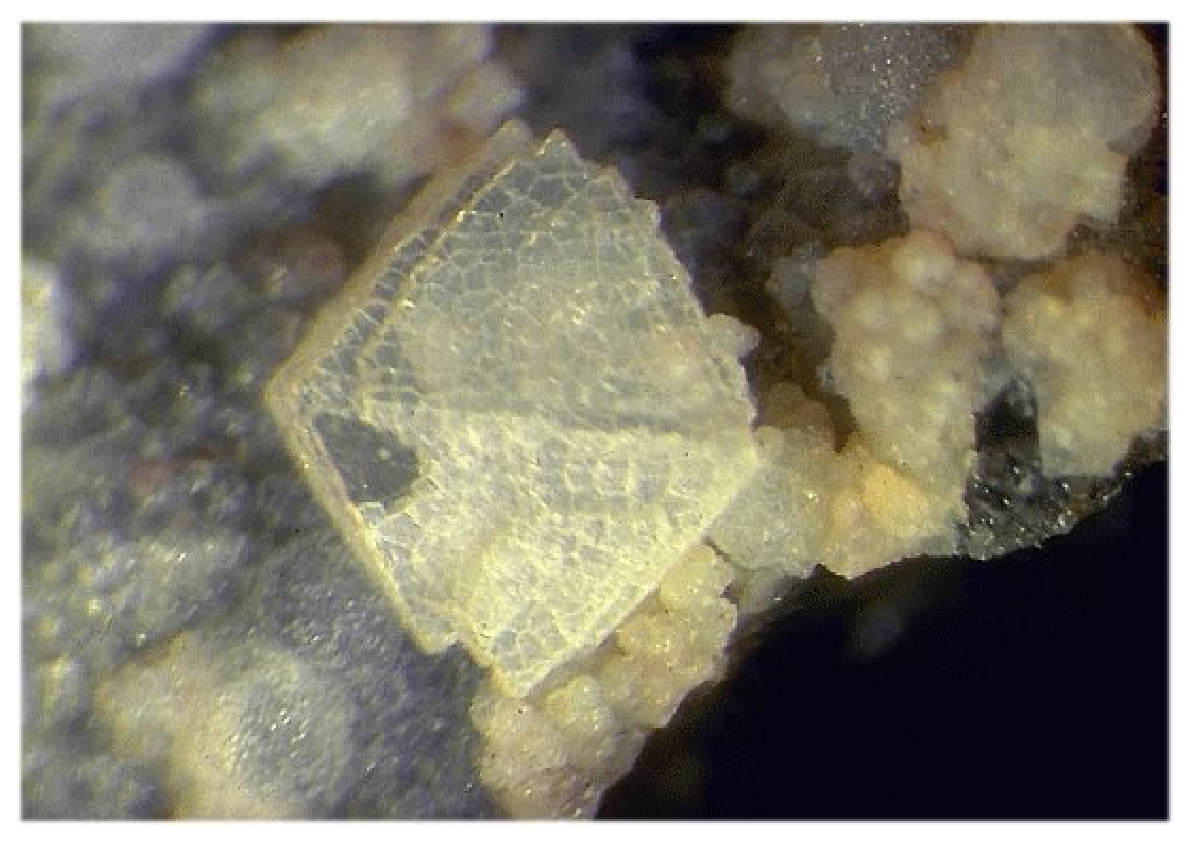
\includegraphics[width=3.5in]{fau-photo.eps}
  \end{center}
\end{frame}

\begin{frame}
  \begin{center}
    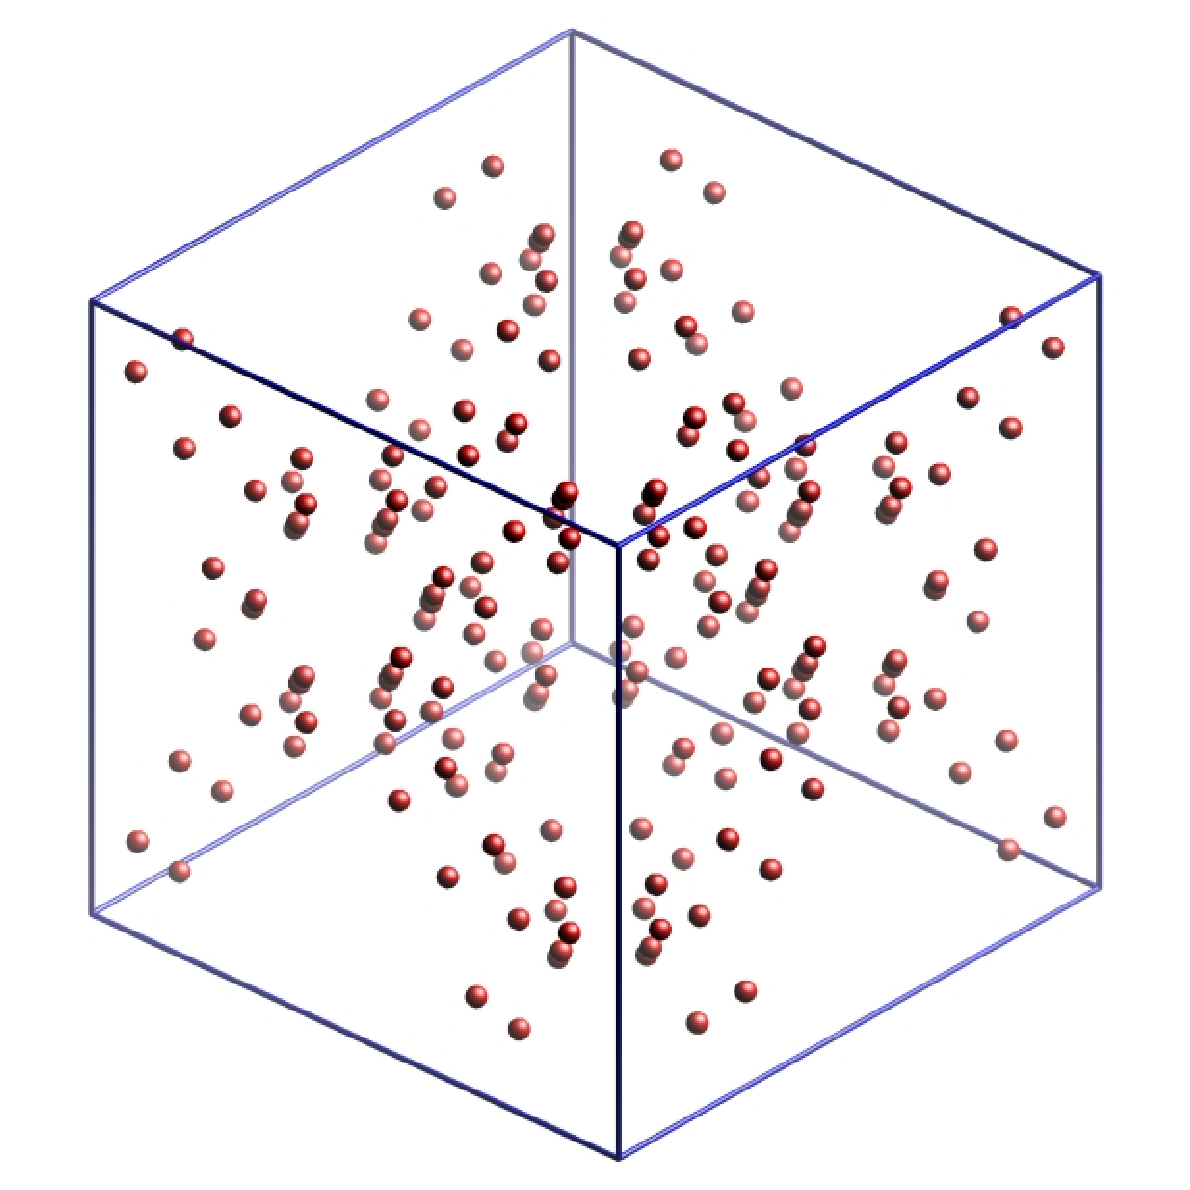
\includegraphics[height=3.5in]{fau-atoms.eps}
  \end{center}
\end{frame}

\begin{frame}
  \begin{center}
    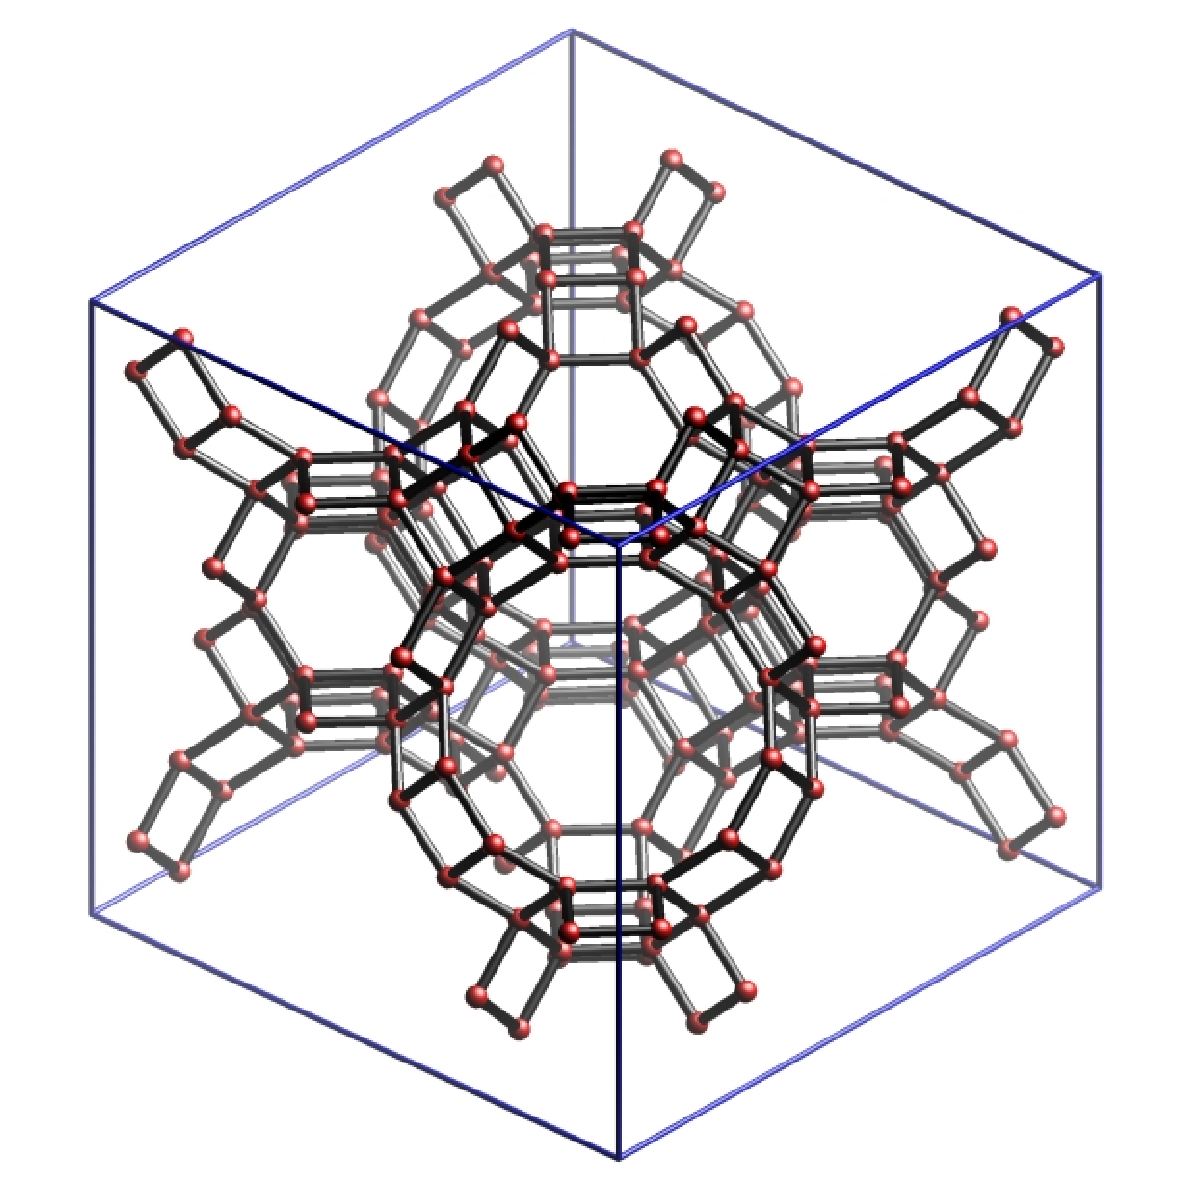
\includegraphics[height=3.5in]{fau-net.eps}
  \end{center}
\end{frame}

\begin{frame}
  \begin{center}
    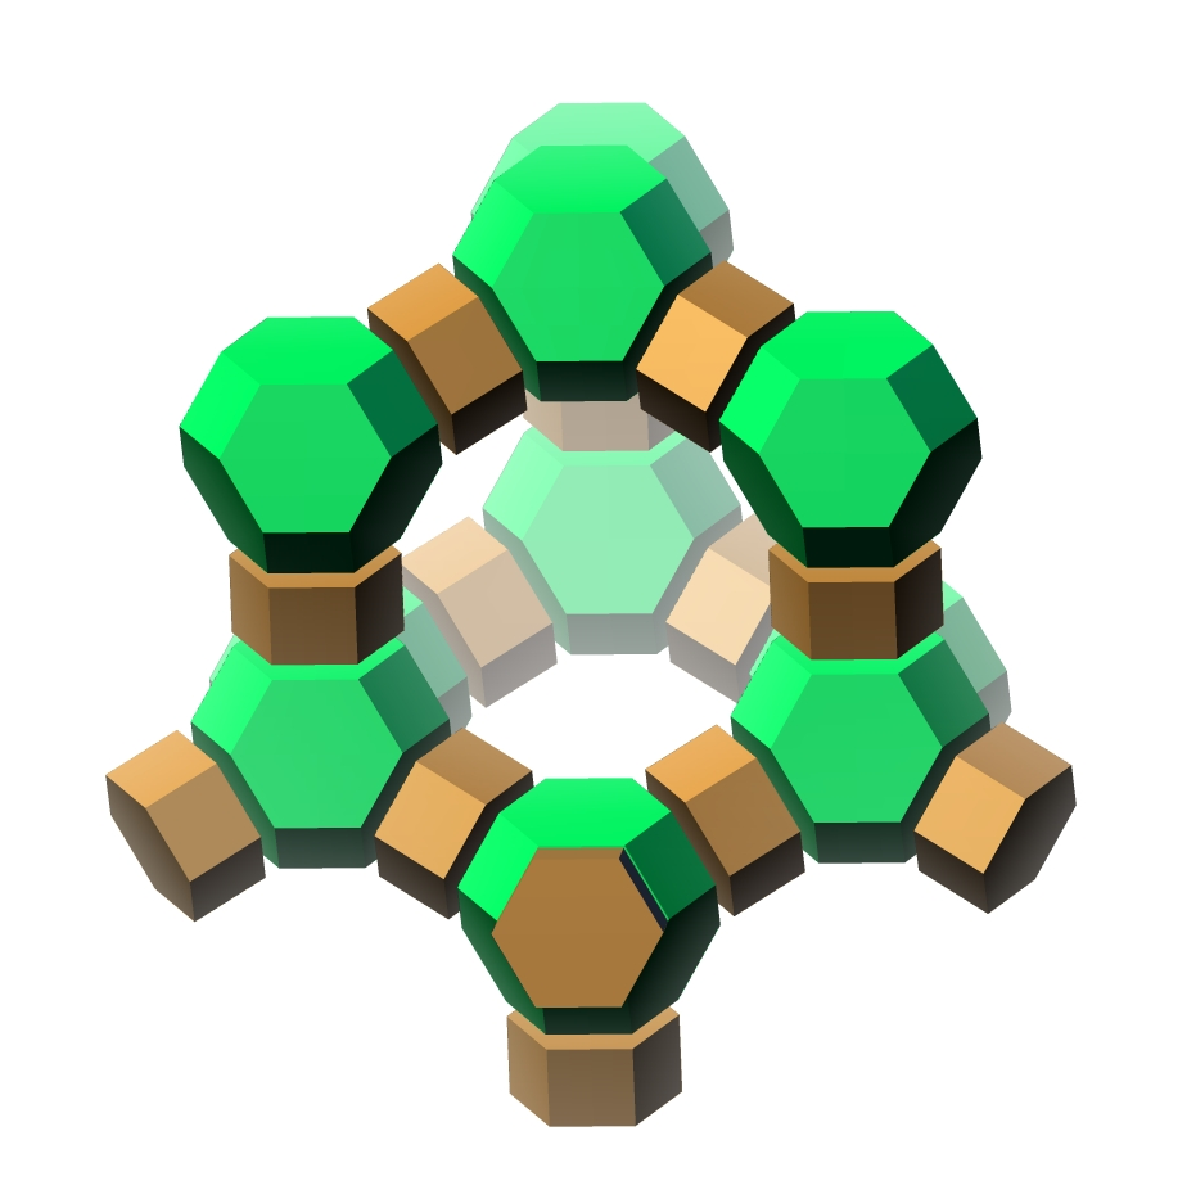
\includegraphics[height=3.5in]{fau-cages.eps}
  \end{center}
\end{frame}

\begin{frame}
  \begin{center}
    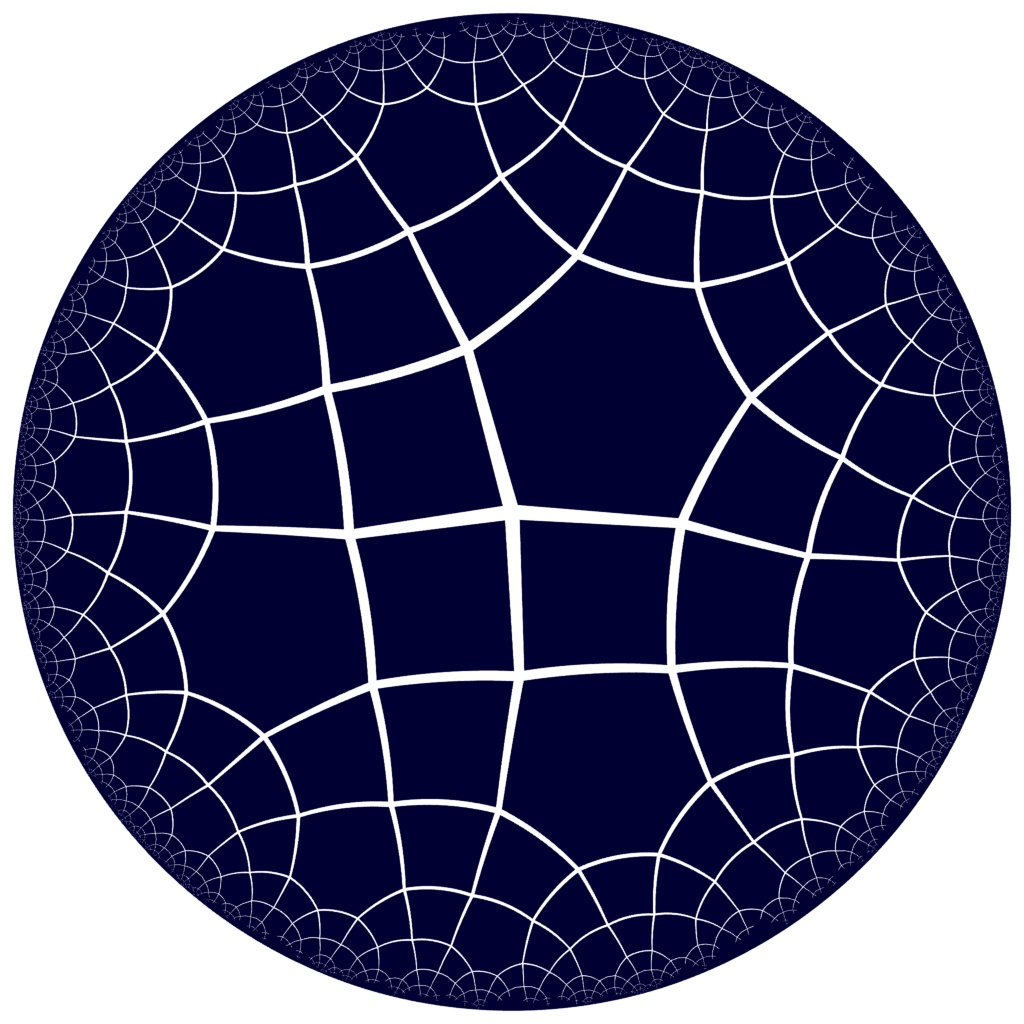
\includegraphics[height=3.5in]{hqc0576.jpg}
  \end{center}
\end{frame}

\begin{frame}
  \begin{center}
    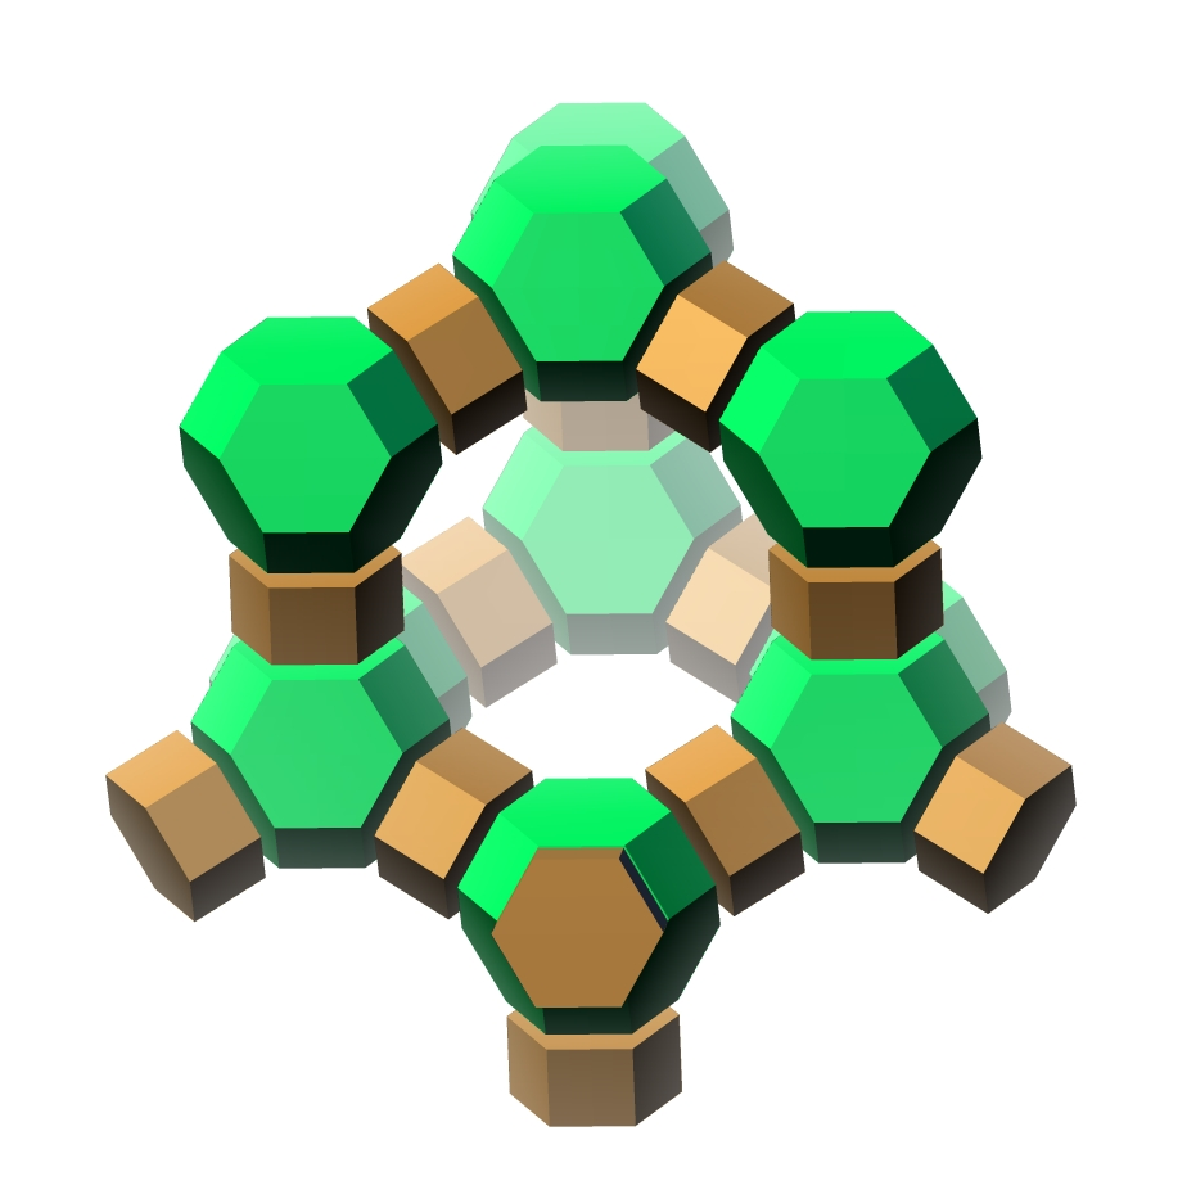
\includegraphics[height=3.5in]{fau-cages.eps}
  \end{center}
\end{frame}

\begin{frame}
  \begin{center}
    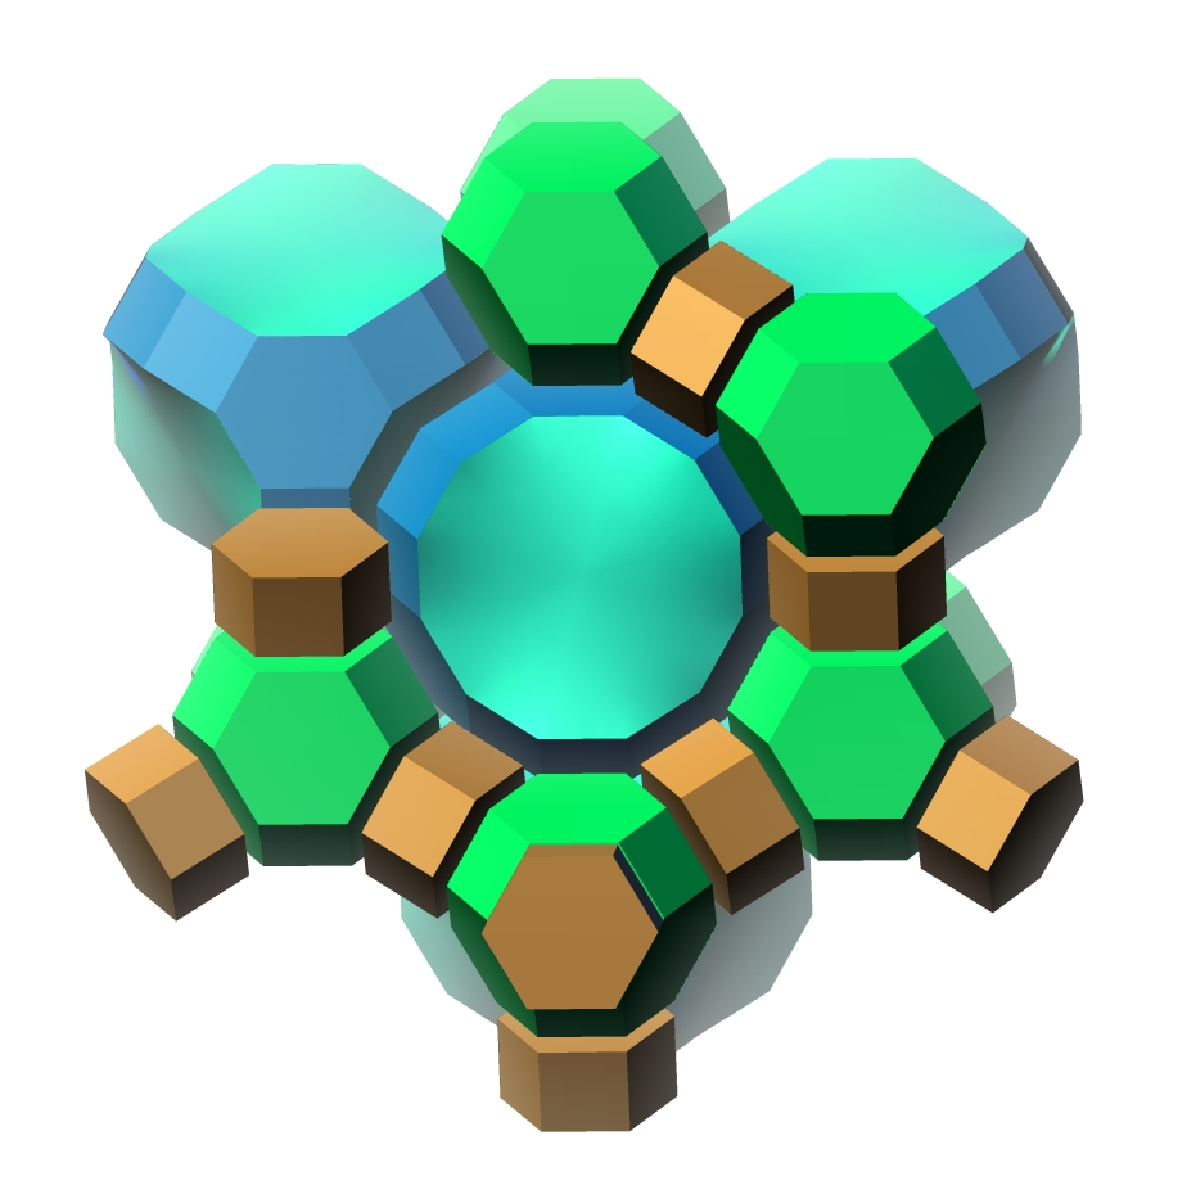
\includegraphics[height=3.5in]{fau-tiling}
  \end{center}
\end{frame}


\section{Periodic Tilings}

\begin{frame}
  \begin{center}
    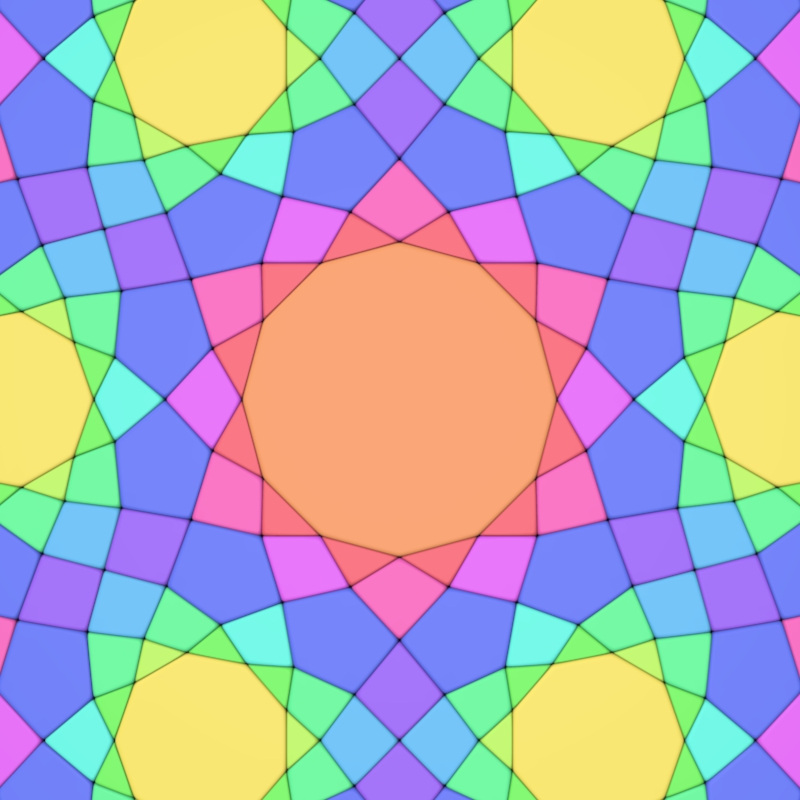
\includegraphics[height=3.5in]{alhambra}
  \end{center}
\end{frame}

\begin{frame}
  \begin{center}
    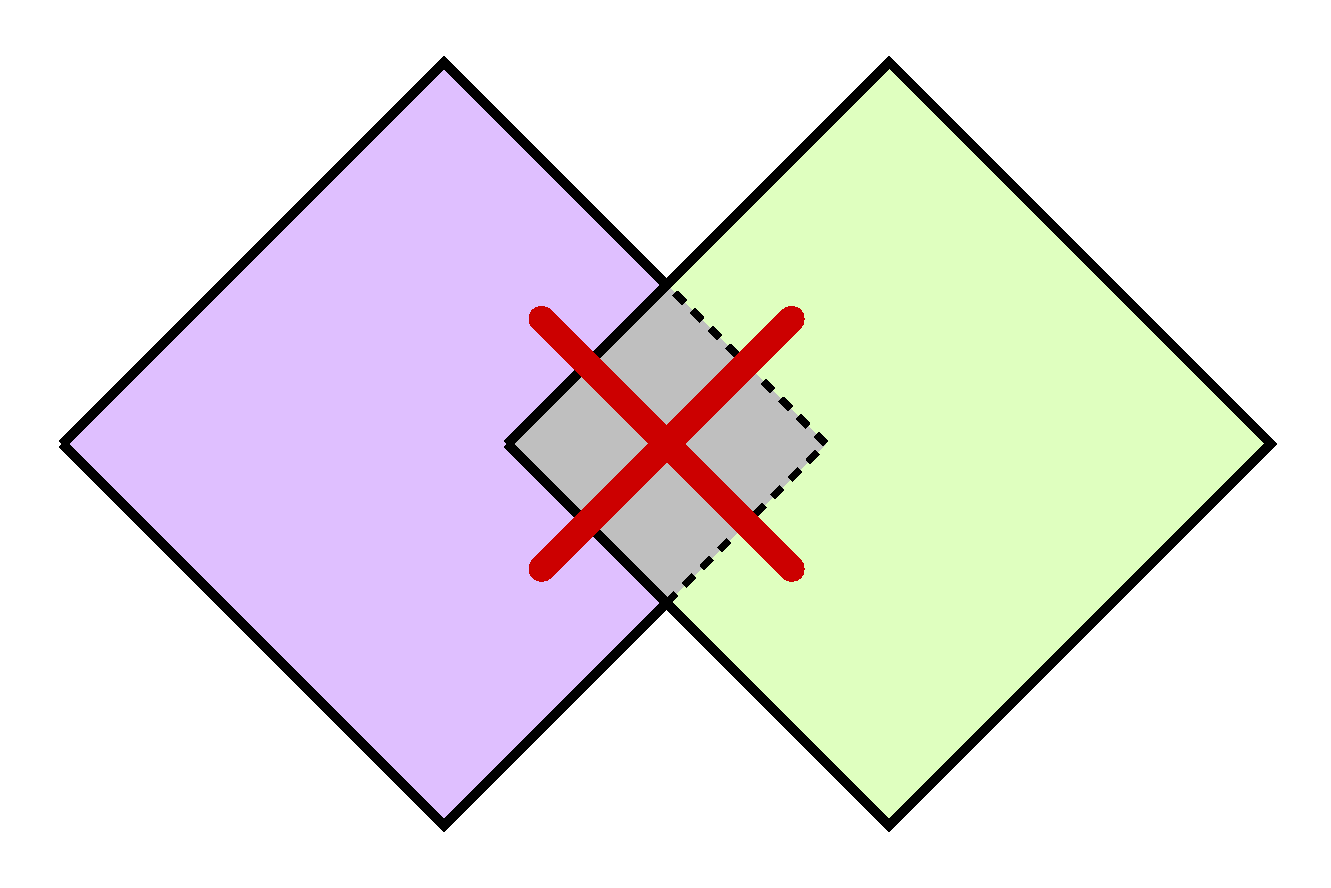
\includegraphics[width=3.5in]{overlaps}
  \end{center}
\end{frame}

\begin{frame}
  \begin{center}
    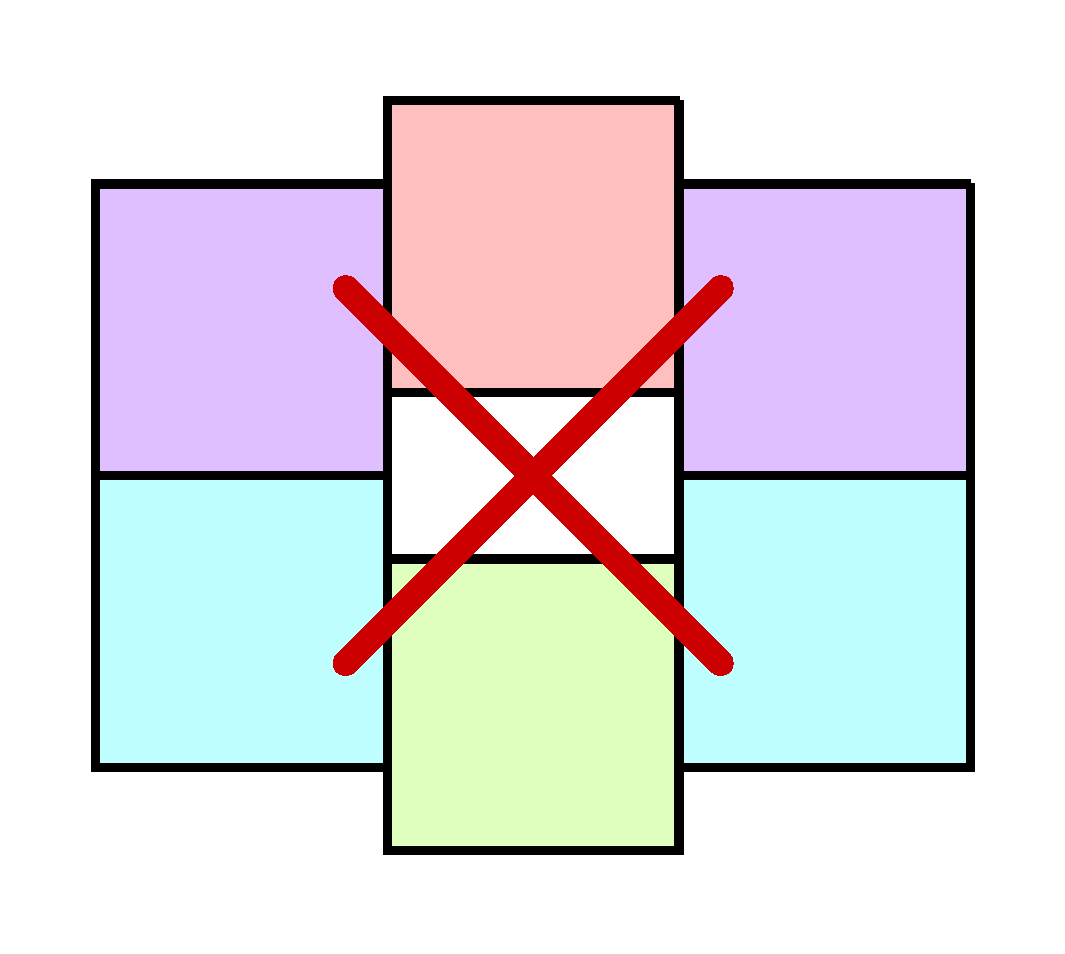
\includegraphics[width=3.5in]{holes}
  \end{center}
\end{frame}

\begin{frame}
  \begin{center}
    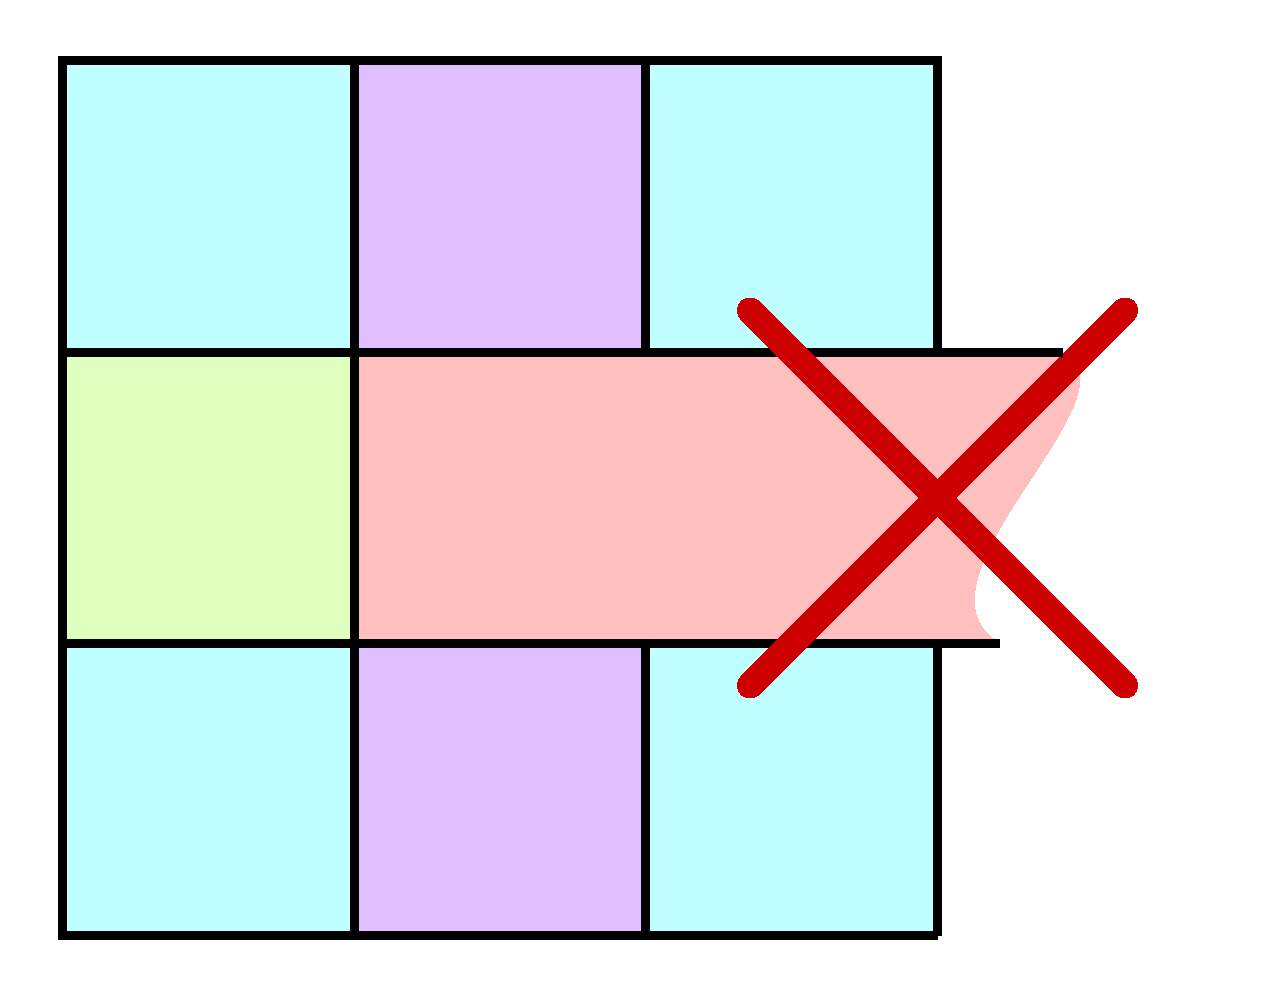
\includegraphics[width=3.5in]{nonbounded}
  \end{center}
\end{frame}

\begin{frame}
  \begin{center}
    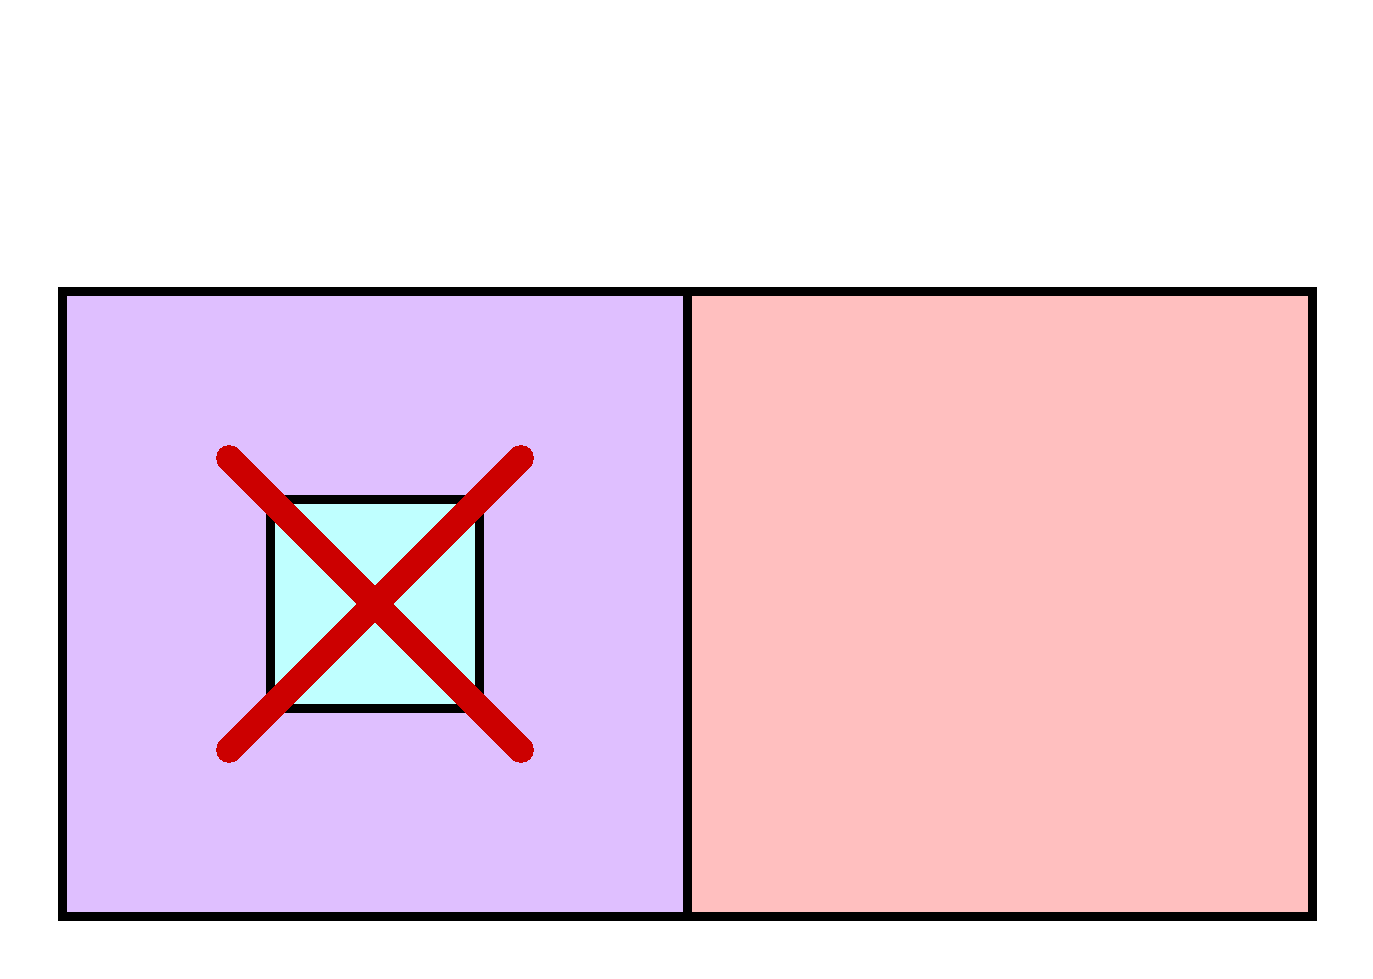
\includegraphics[width=3.5in]{noncell}
  \end{center}
\end{frame}

\begin{frame}
  \begin{center}
    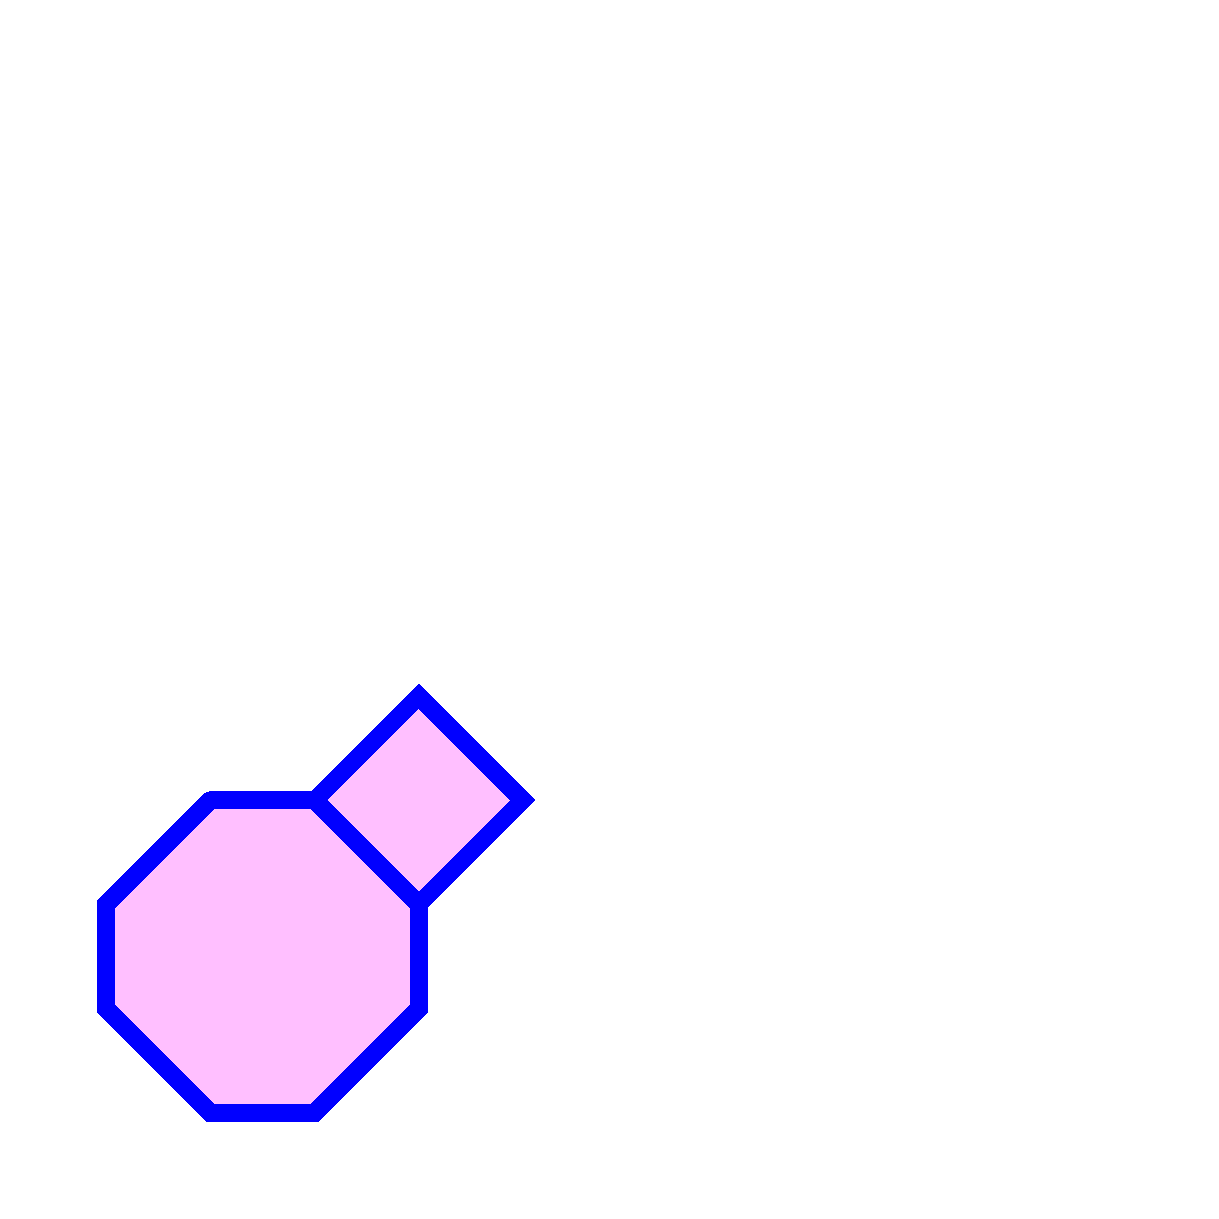
\includegraphics[width=3.5in]{periodic1}
  \end{center}
\end{frame}

\begin{frame}
  \begin{center}
    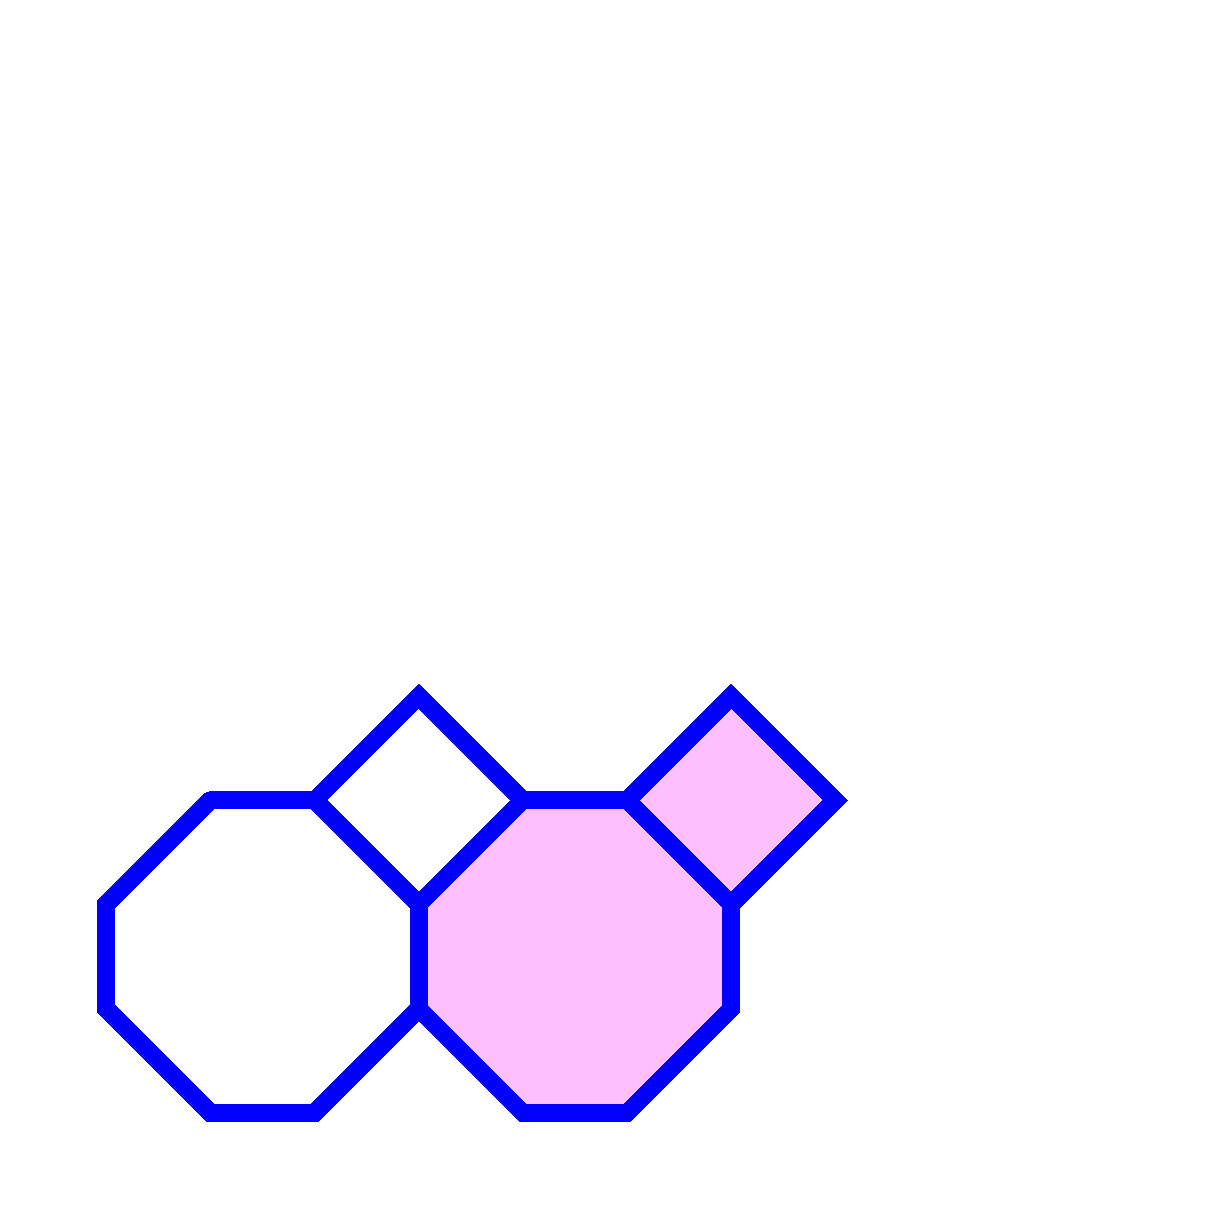
\includegraphics[width=3.5in]{periodic2}
  \end{center}
\end{frame}

\begin{frame}
  \begin{center}
    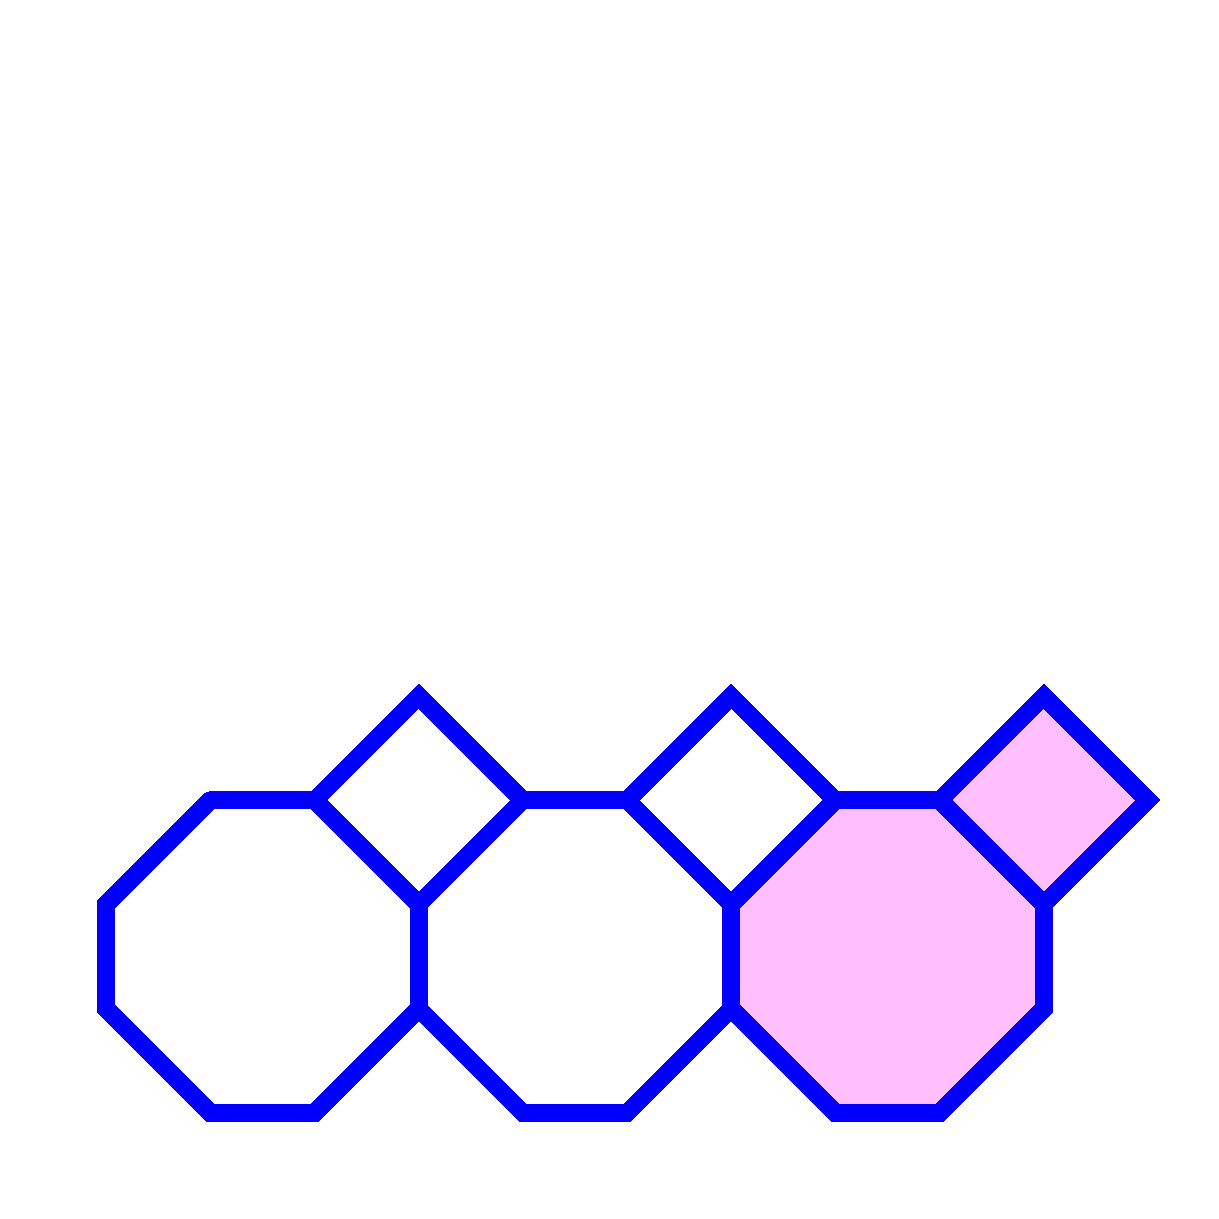
\includegraphics[width=3.5in]{periodic3}
  \end{center}
\end{frame}

\begin{frame}
  \begin{center}
    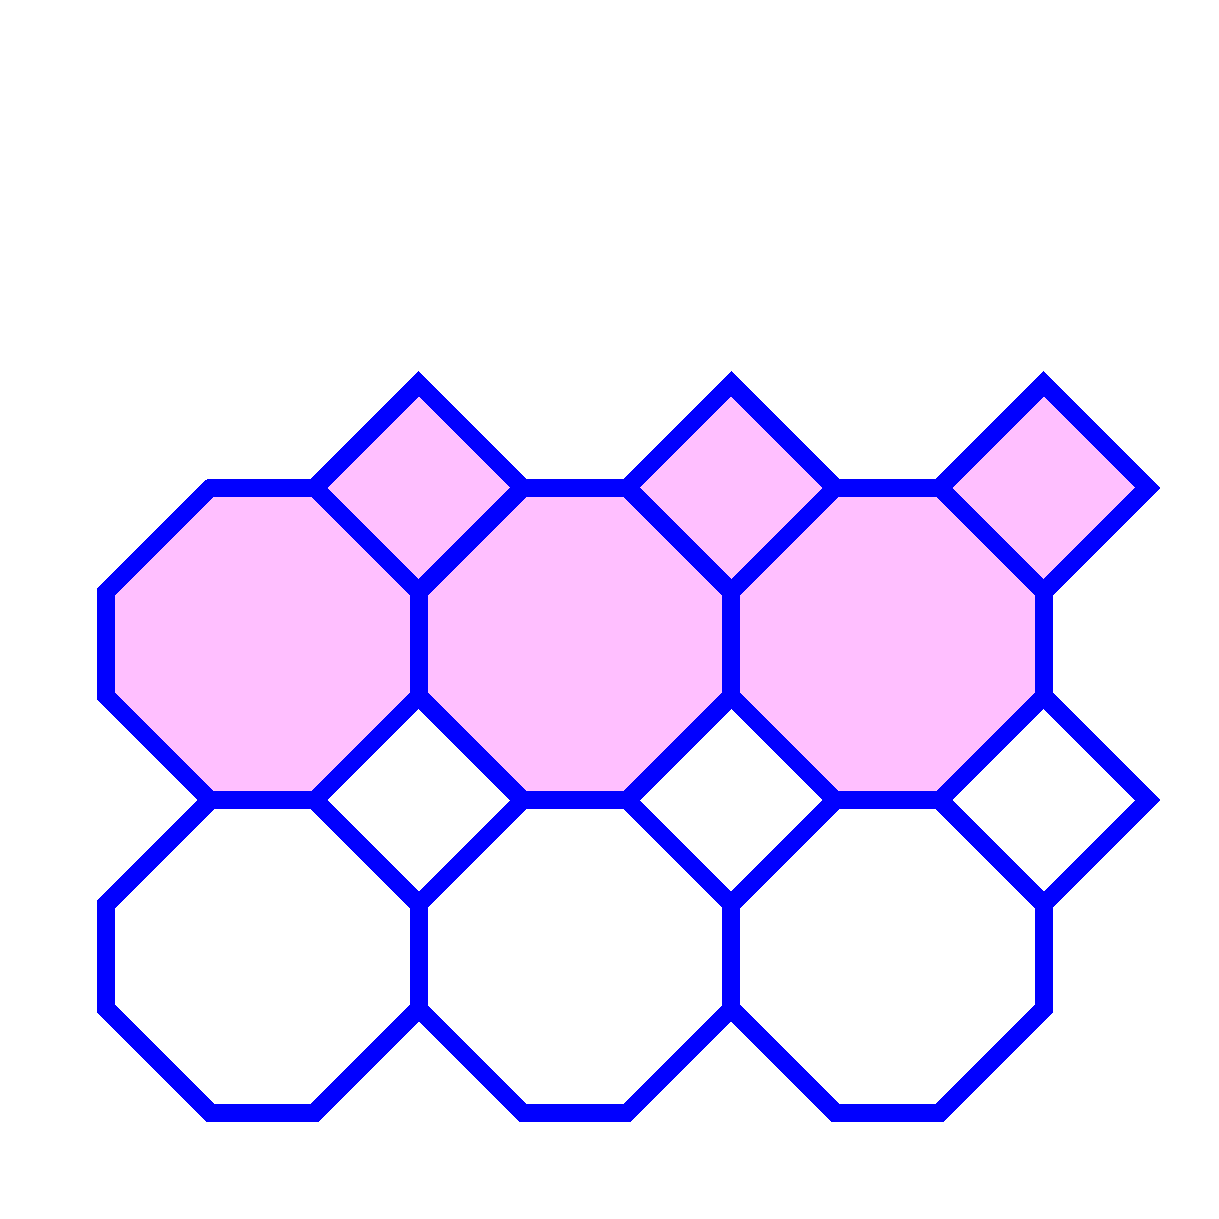
\includegraphics[width=3.5in]{periodic4}
  \end{center}
\end{frame}

\begin{frame}
  \begin{center}
    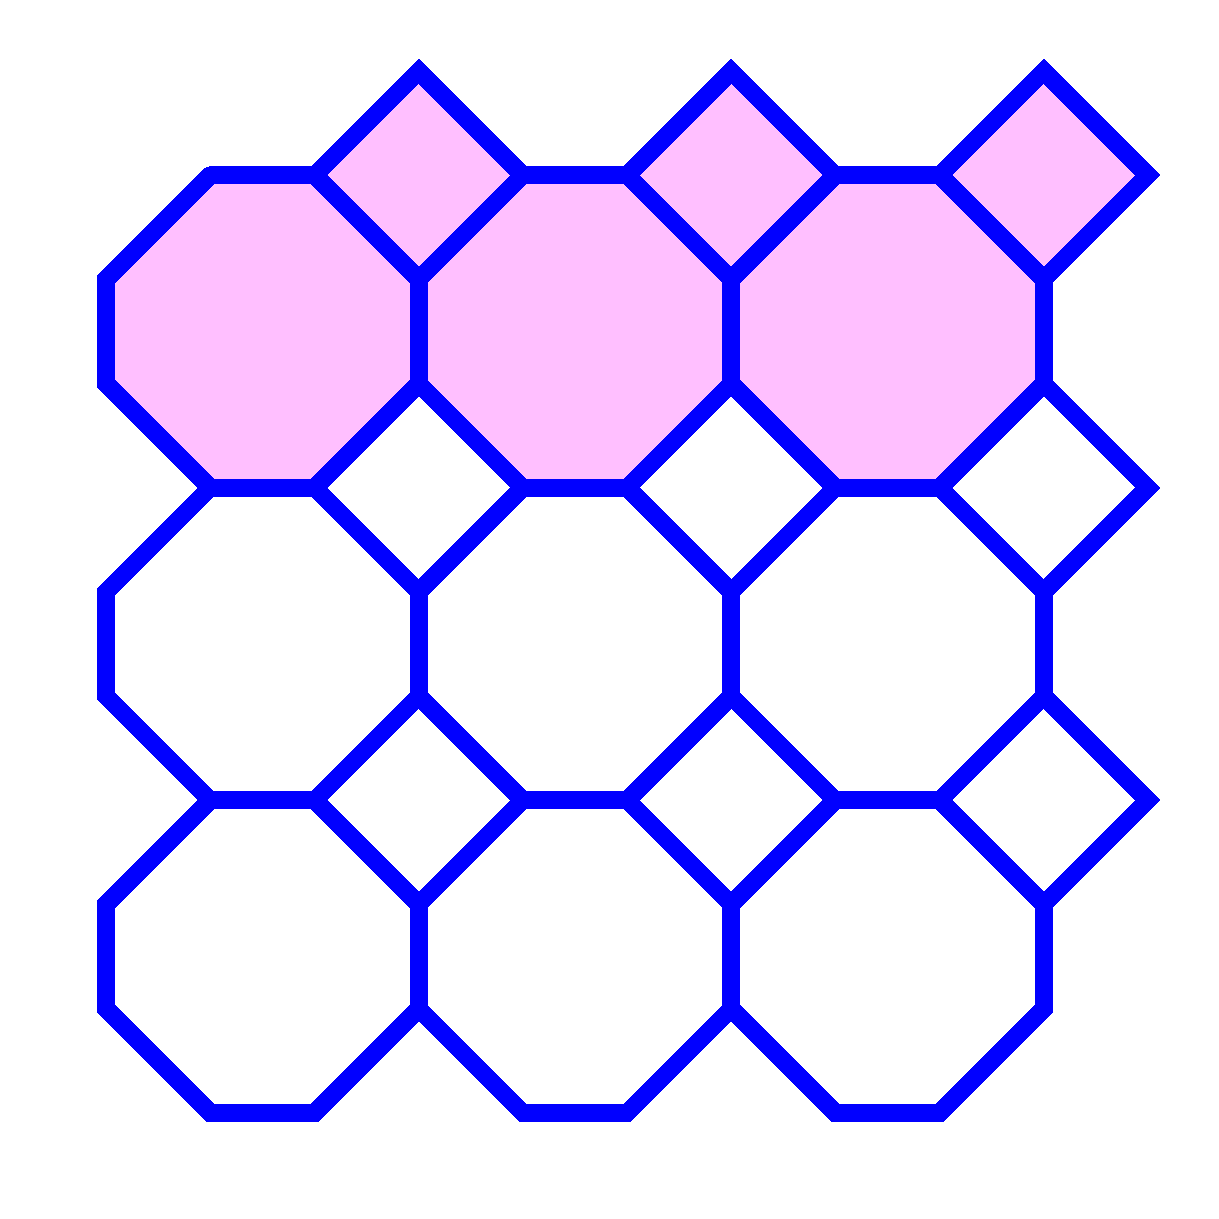
\includegraphics[width=3.5in]{periodic5}
  \end{center}
\end{frame}

\begin{frame}
  \begin{center}
    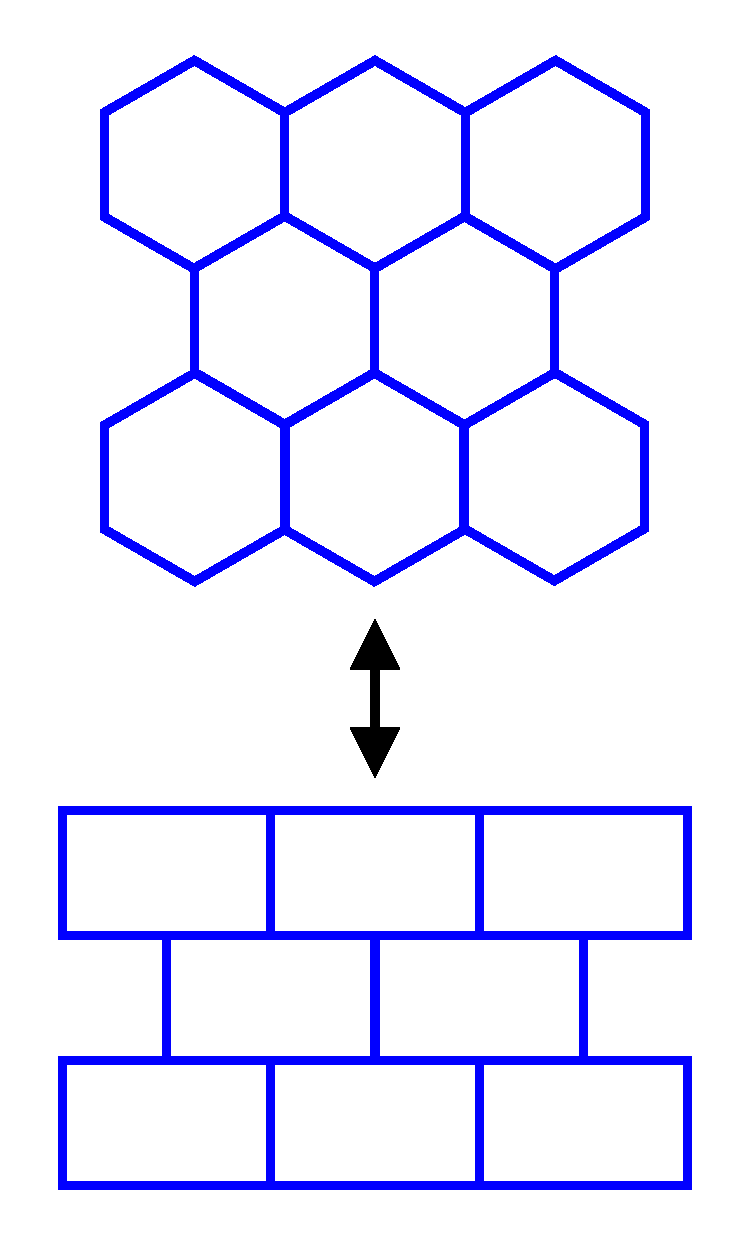
\includegraphics[height=3.5in]{topol-equiv-alt}
  \end{center}
\end{frame}

\begin{frame}
  \begin{center}
    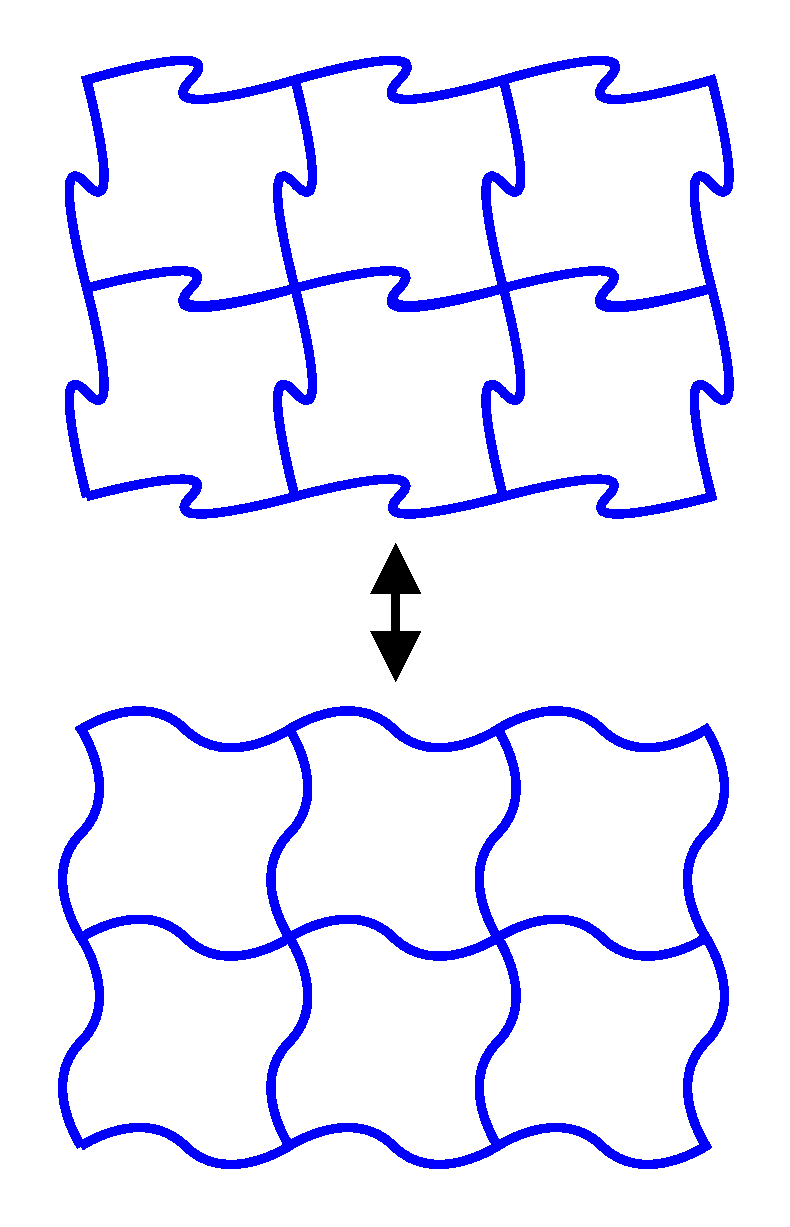
\includegraphics[height=3.5in]{equiv-equiv-alt}
  \end{center}
\end{frame}


\section{Another Collatz Problem}

\begin{frame}
  \begin{center}
    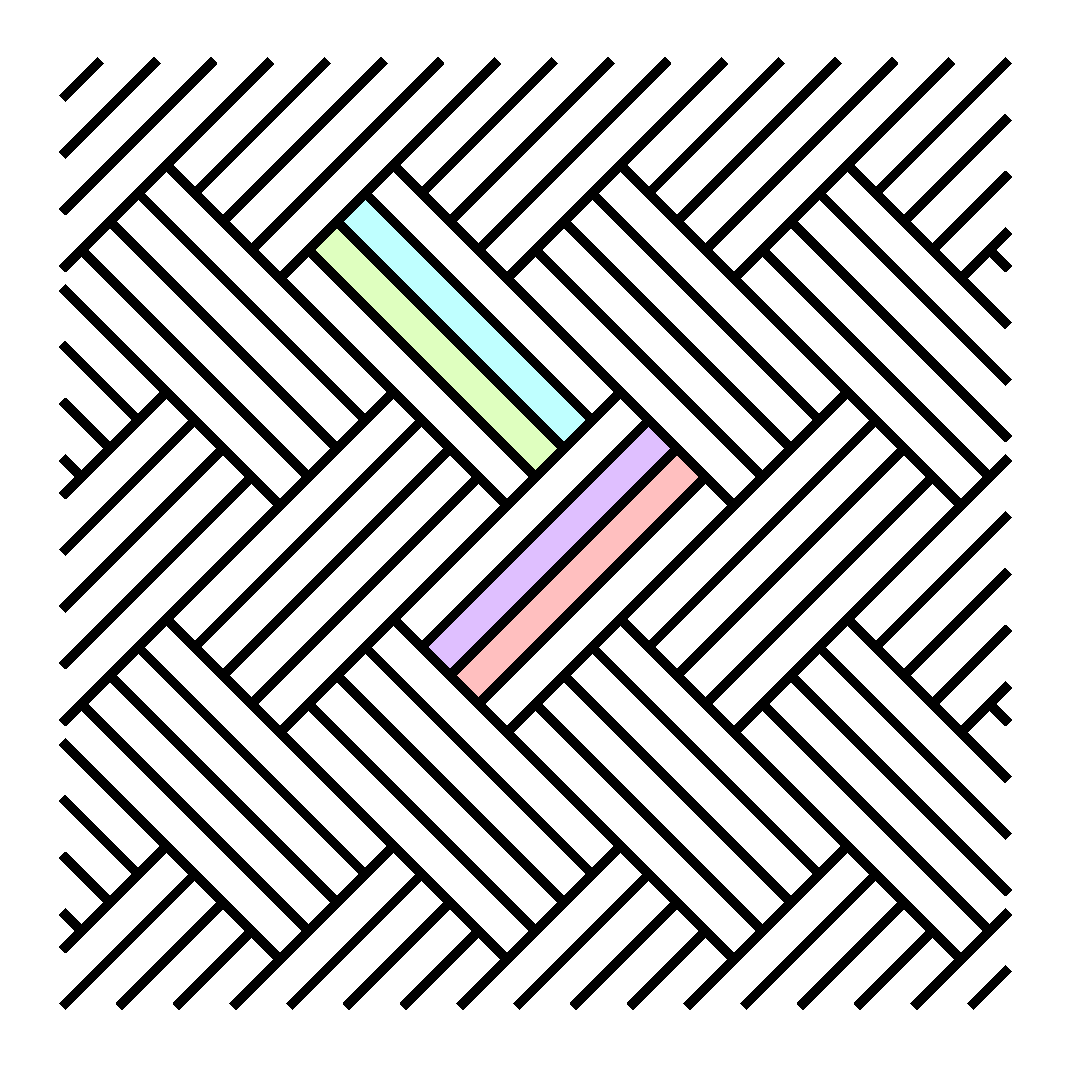
\includegraphics[width=1.9in]{c01}
    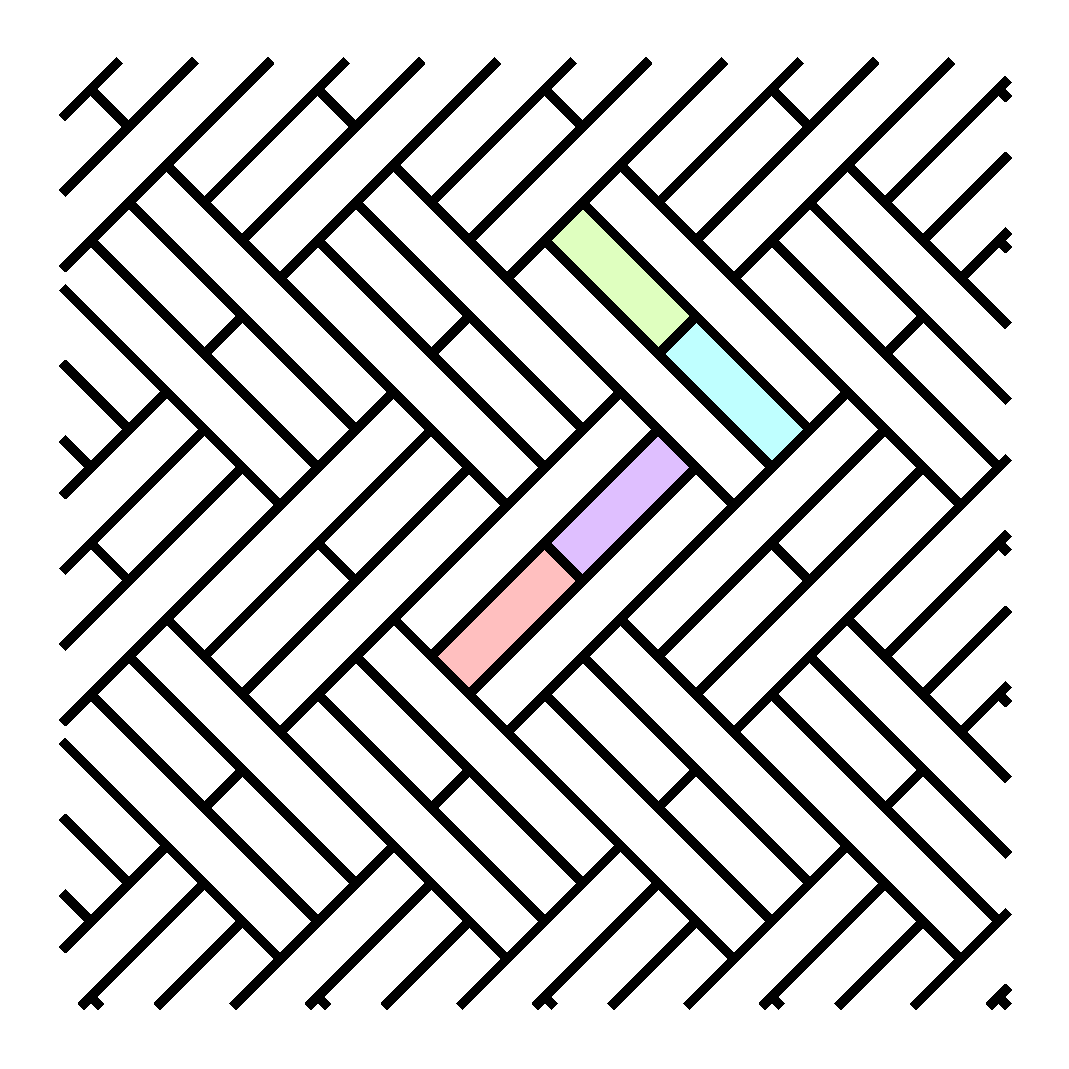
\includegraphics[width=1.9in]{c12}
  \end{center}
\end{frame}

\begin{frame}
  \begin{center}
    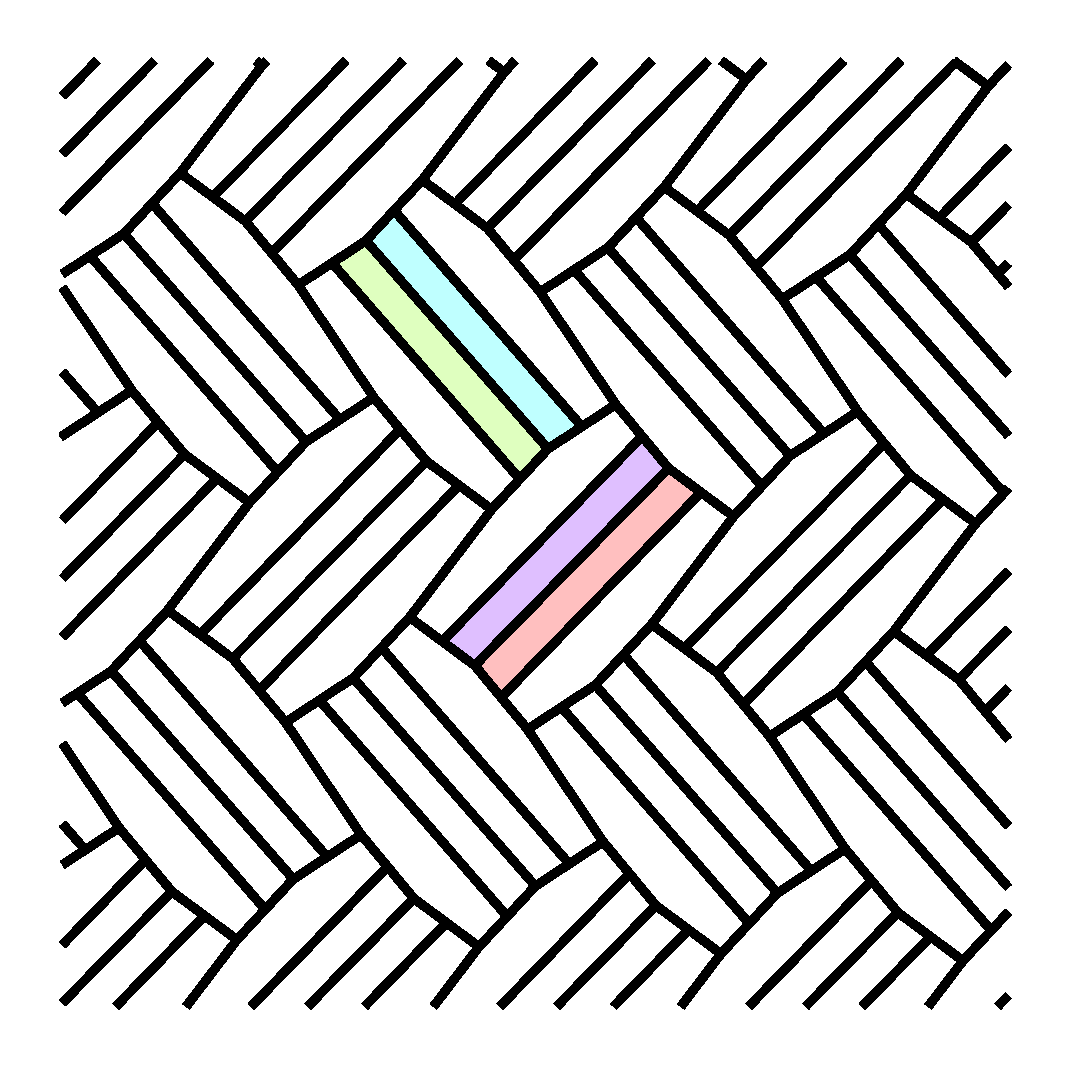
\includegraphics[width=1.9in]{c02}
    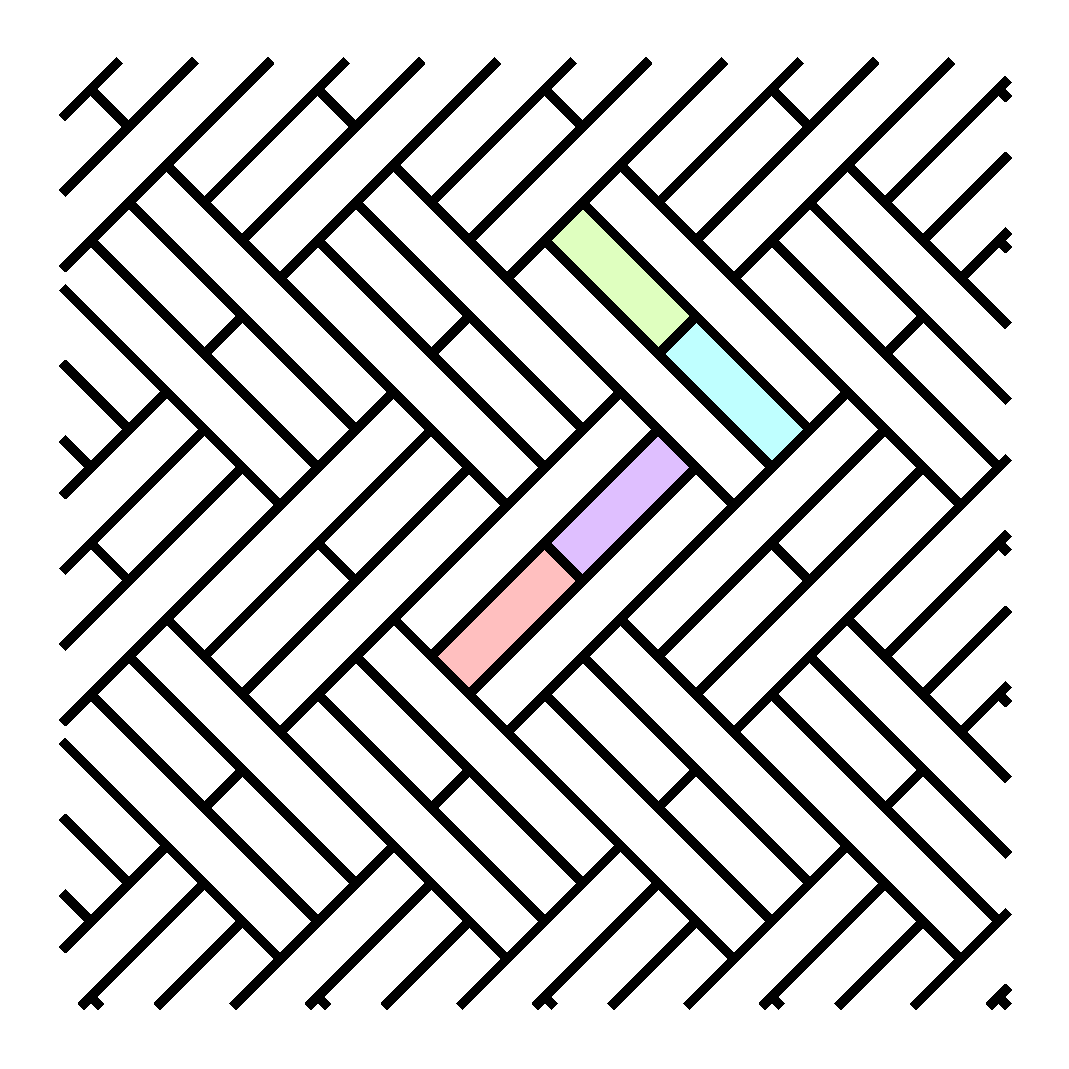
\includegraphics[width=1.9in]{c12}
  \end{center}
\end{frame}

\begin{frame}
  \begin{center}
    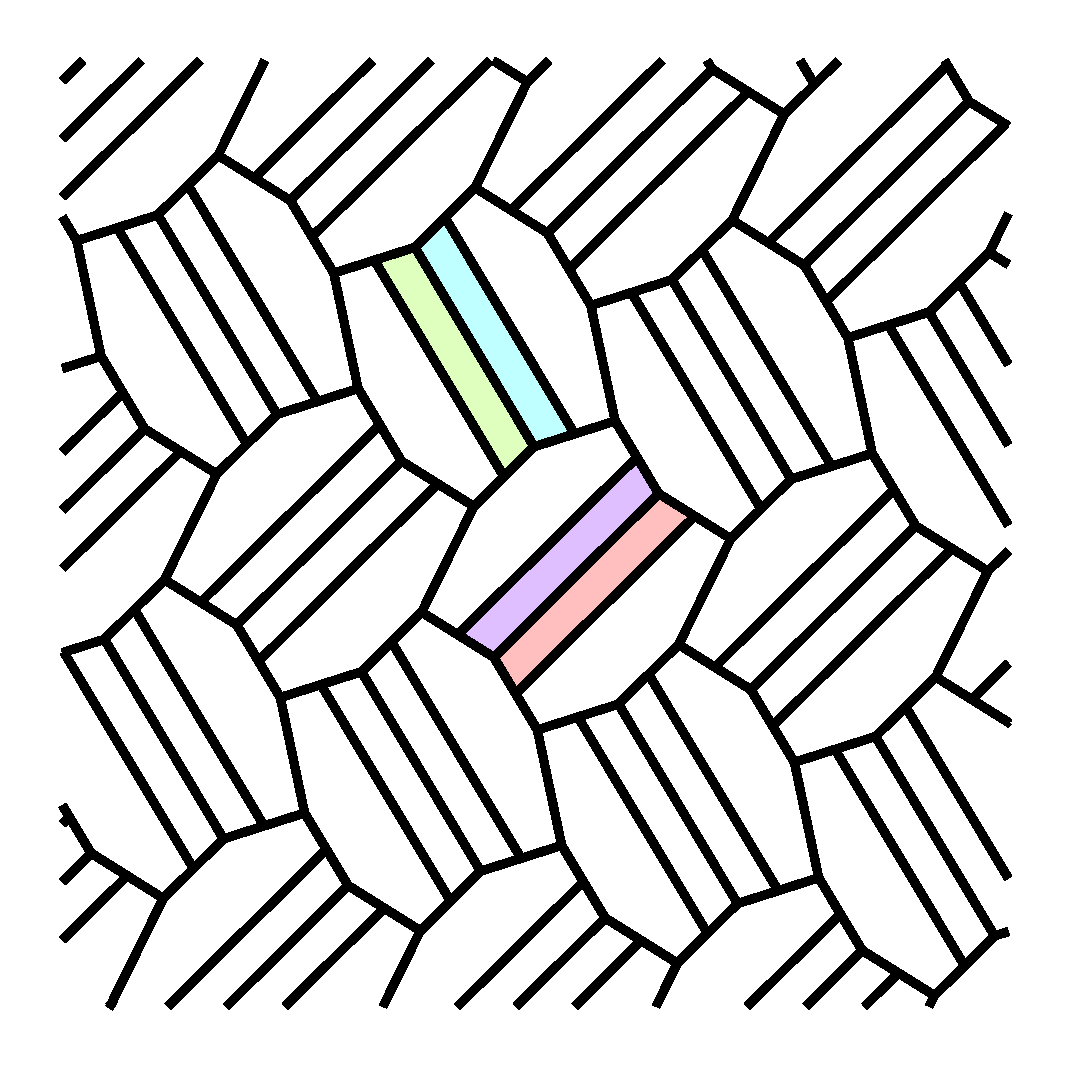
\includegraphics[width=1.9in]{c03}
    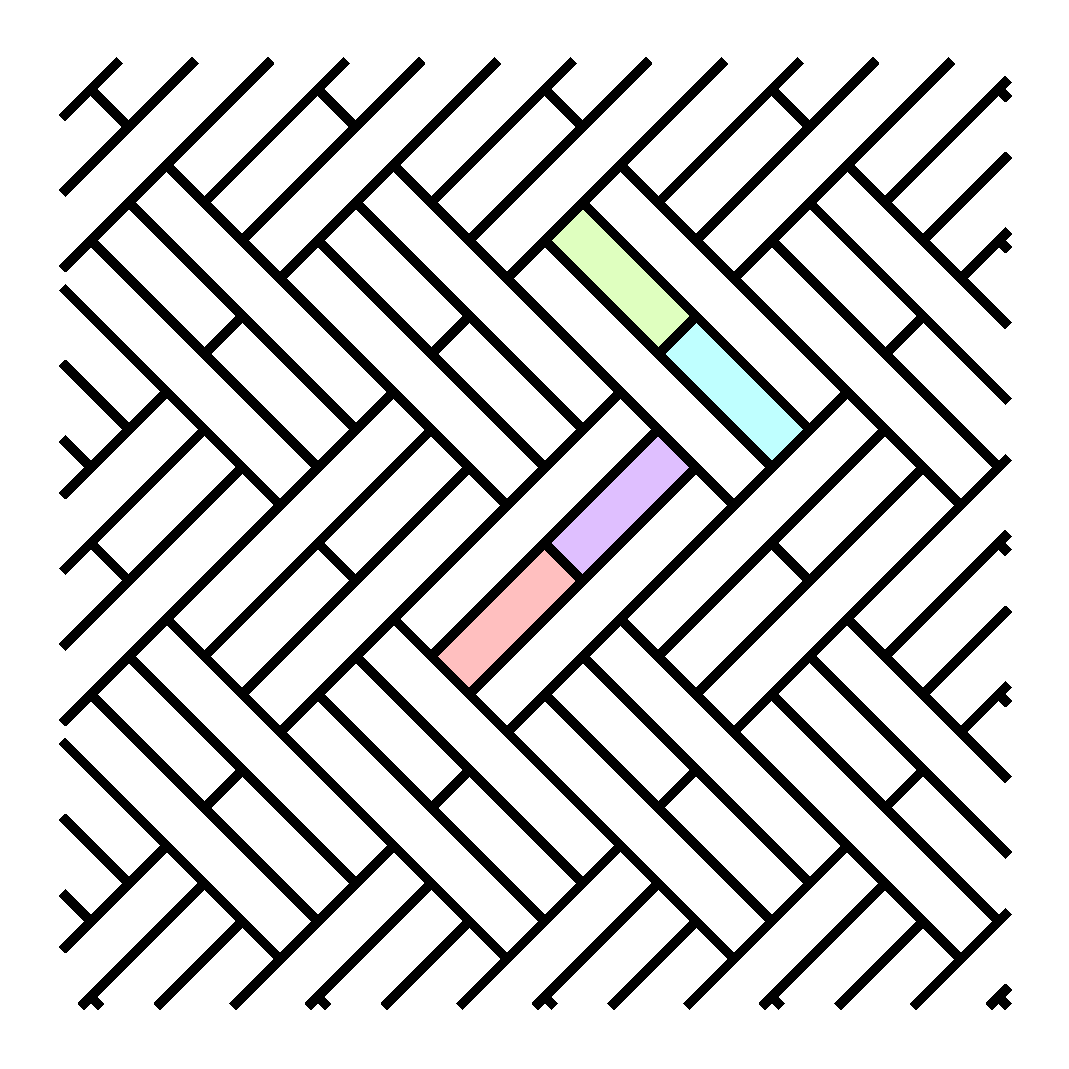
\includegraphics[width=1.9in]{c12}
  \end{center}
\end{frame}

\begin{frame}
  \begin{center}
    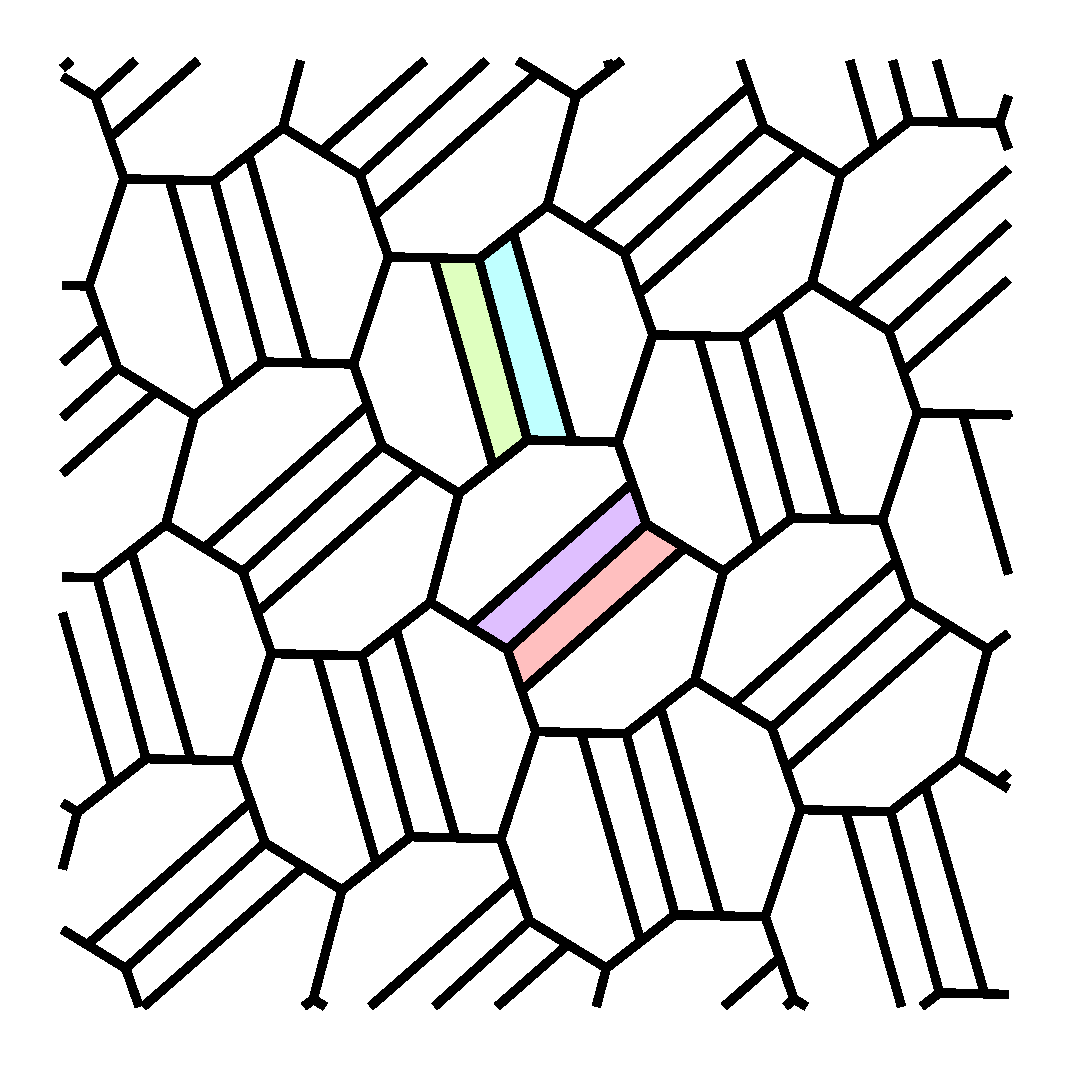
\includegraphics[width=1.9in]{c04}
    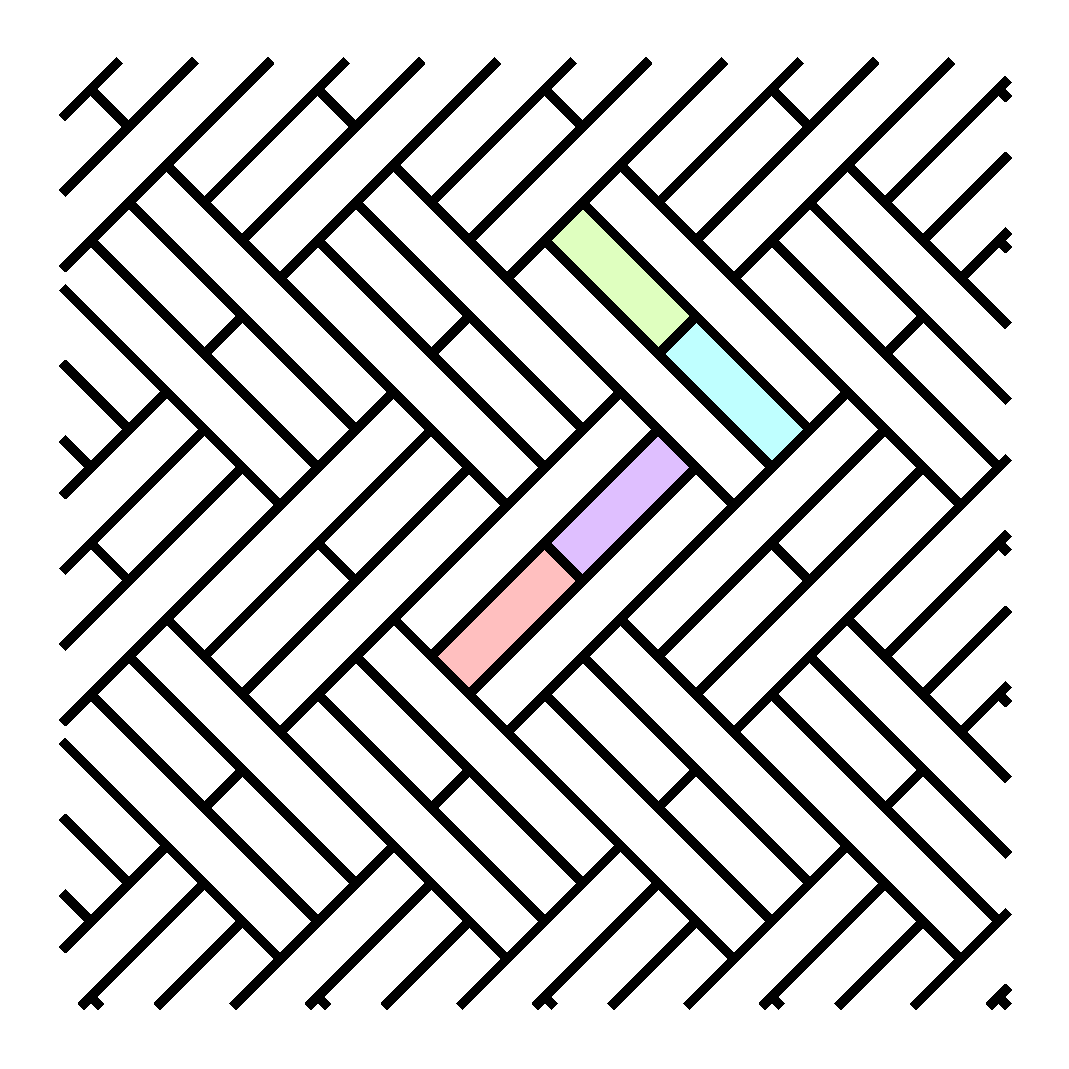
\includegraphics[width=1.9in]{c12}
  \end{center}
\end{frame}

\begin{frame}
  \begin{center}
    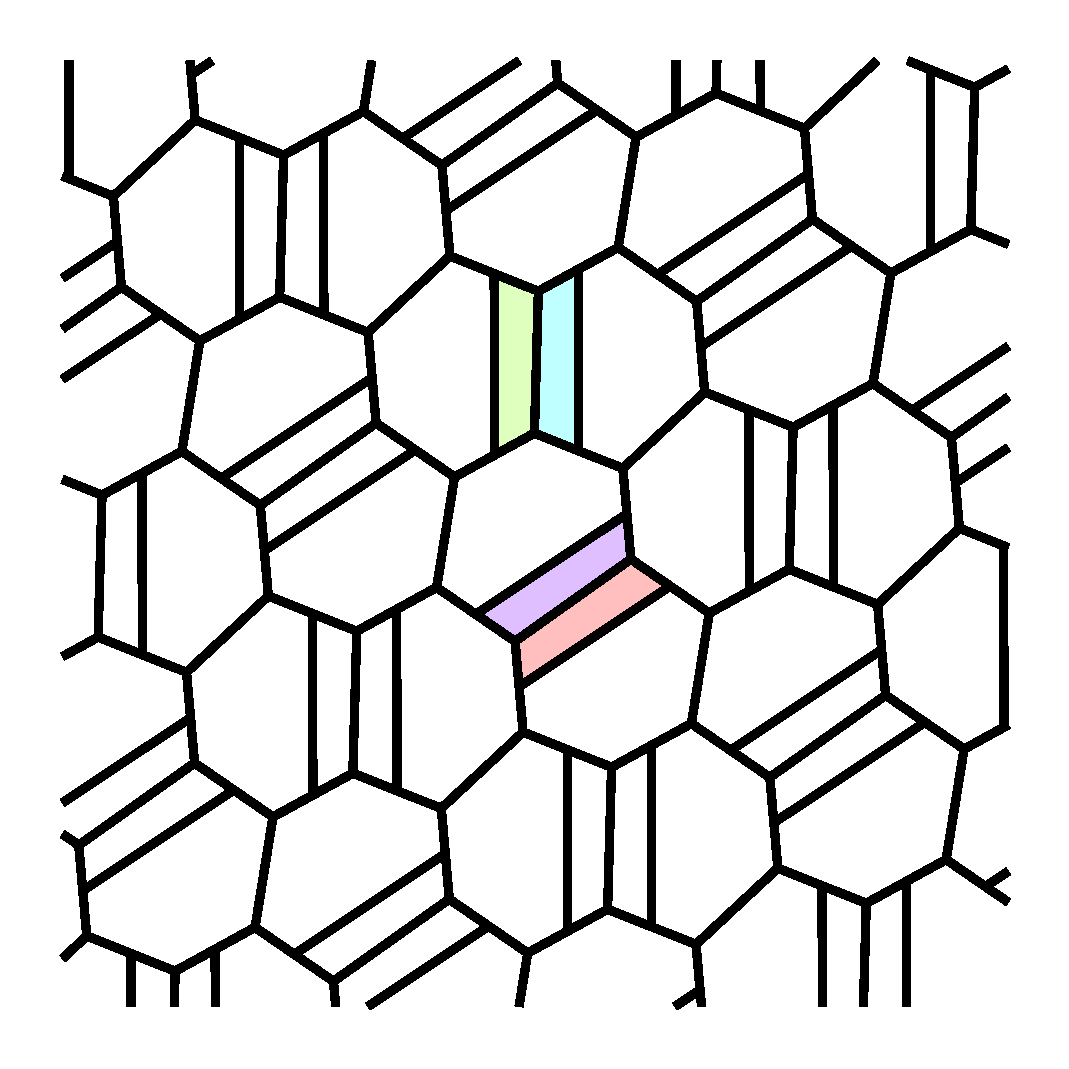
\includegraphics[width=1.9in]{c05}
    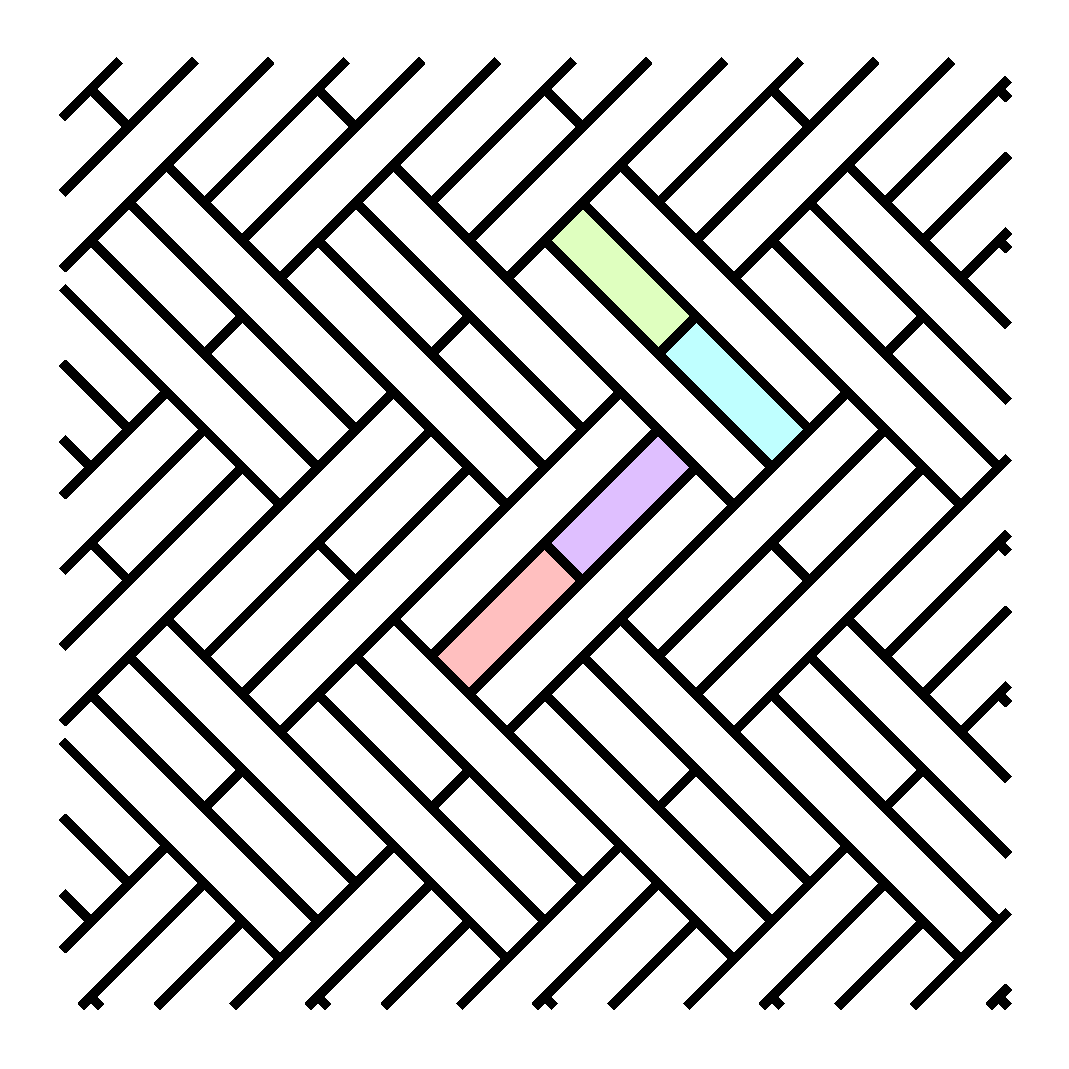
\includegraphics[width=1.9in]{c12}
  \end{center}
\end{frame}

\begin{frame}
  \begin{center}
    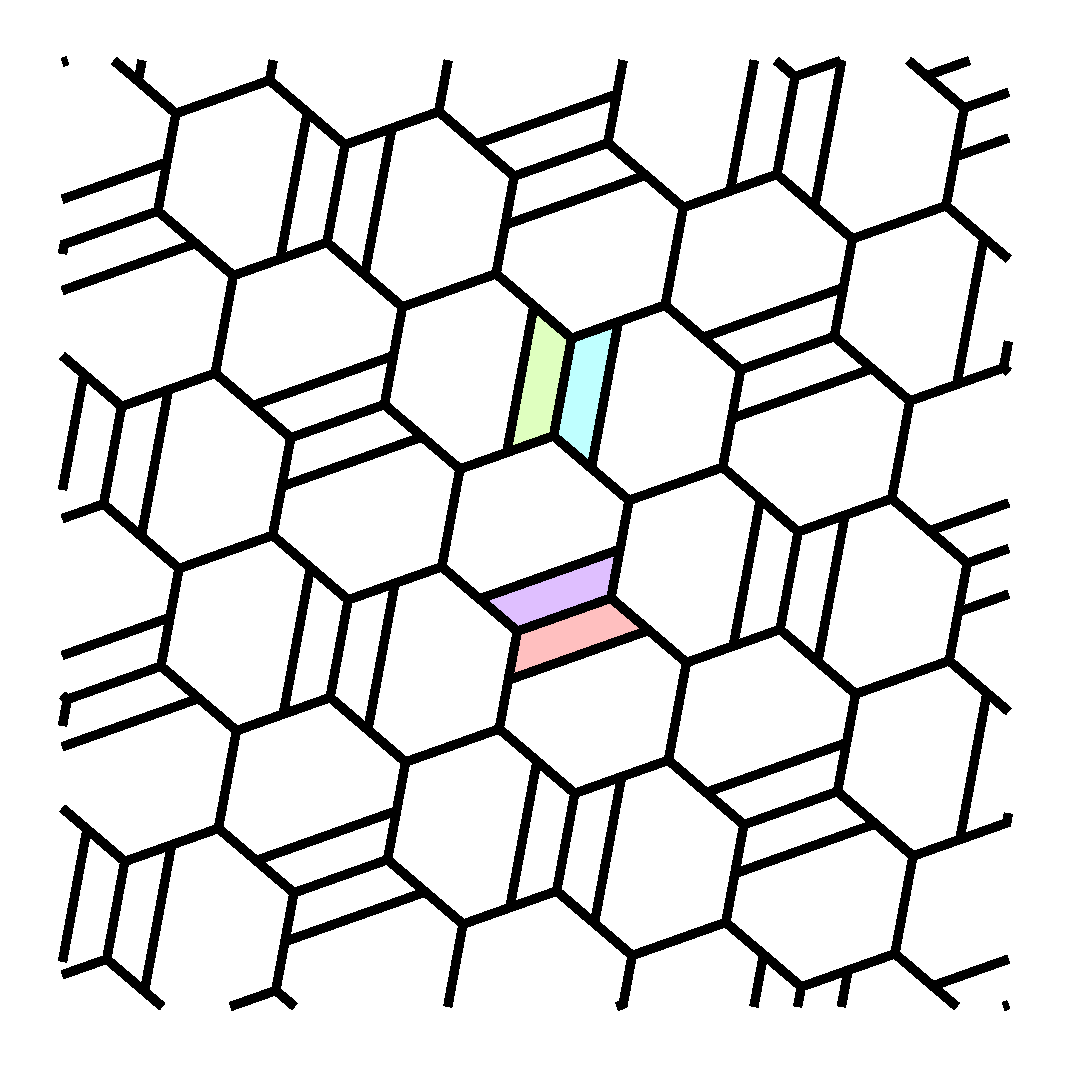
\includegraphics[width=1.9in]{c06}
    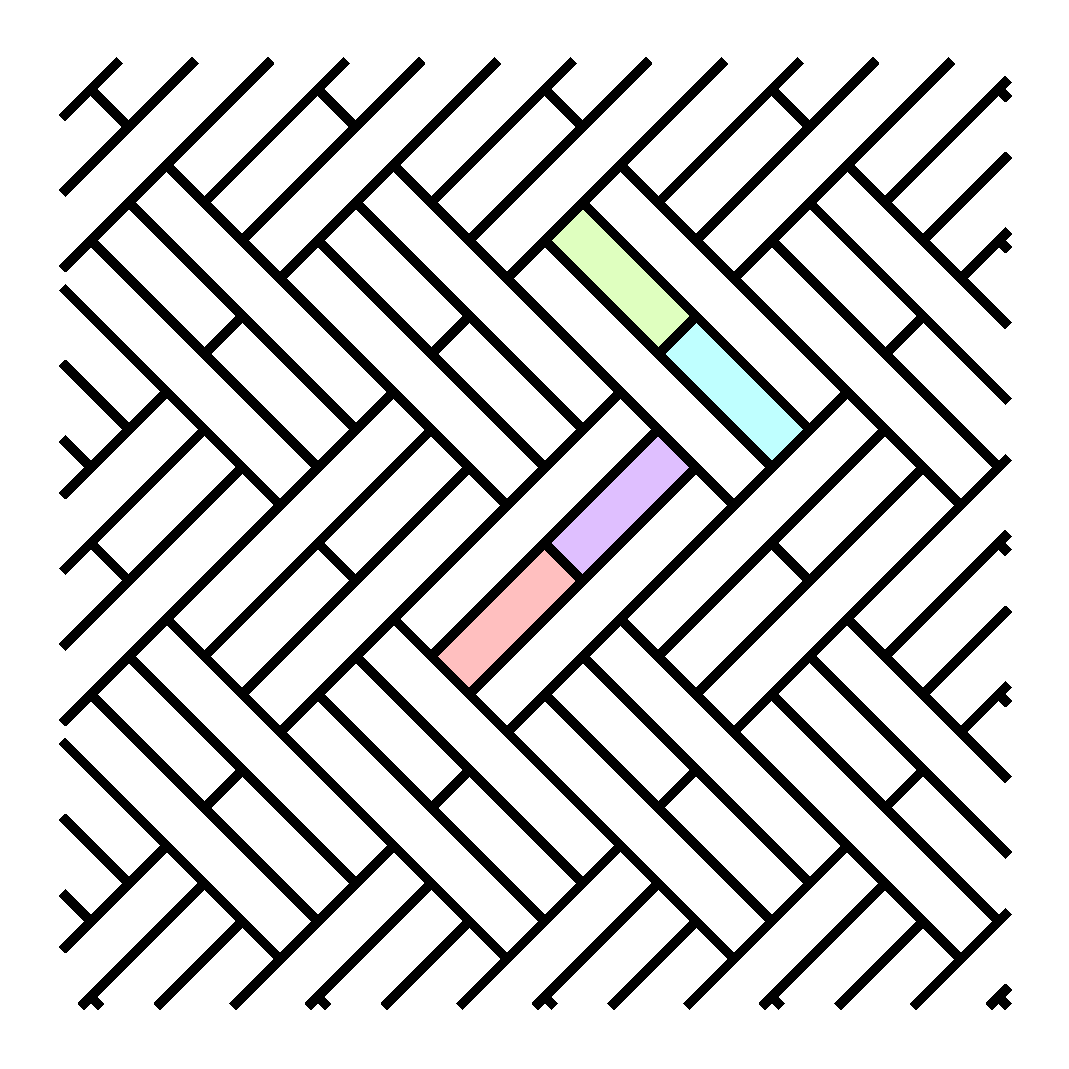
\includegraphics[width=1.9in]{c12}
  \end{center}
\end{frame}

\begin{frame}
  \begin{center}
    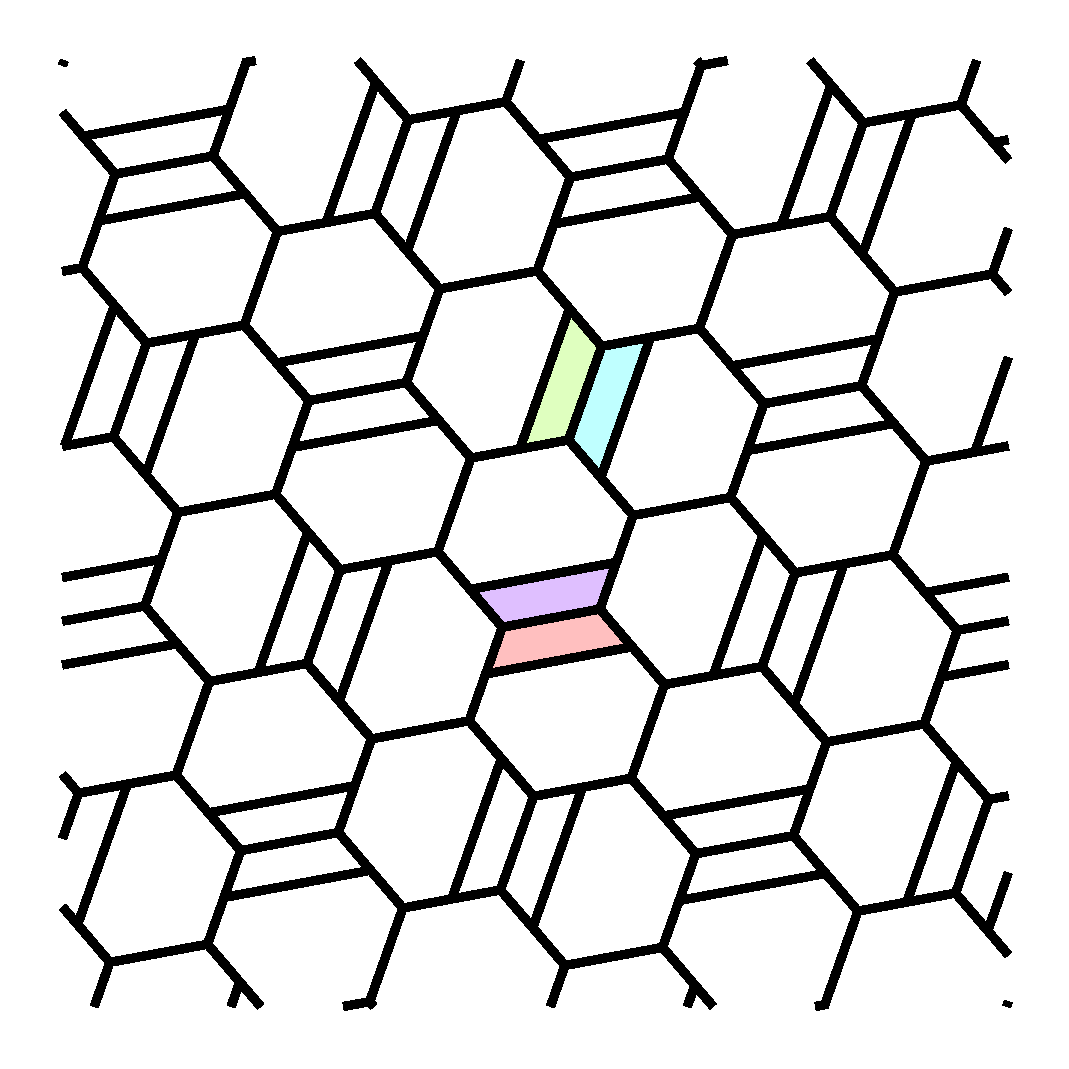
\includegraphics[width=1.9in]{c07}
    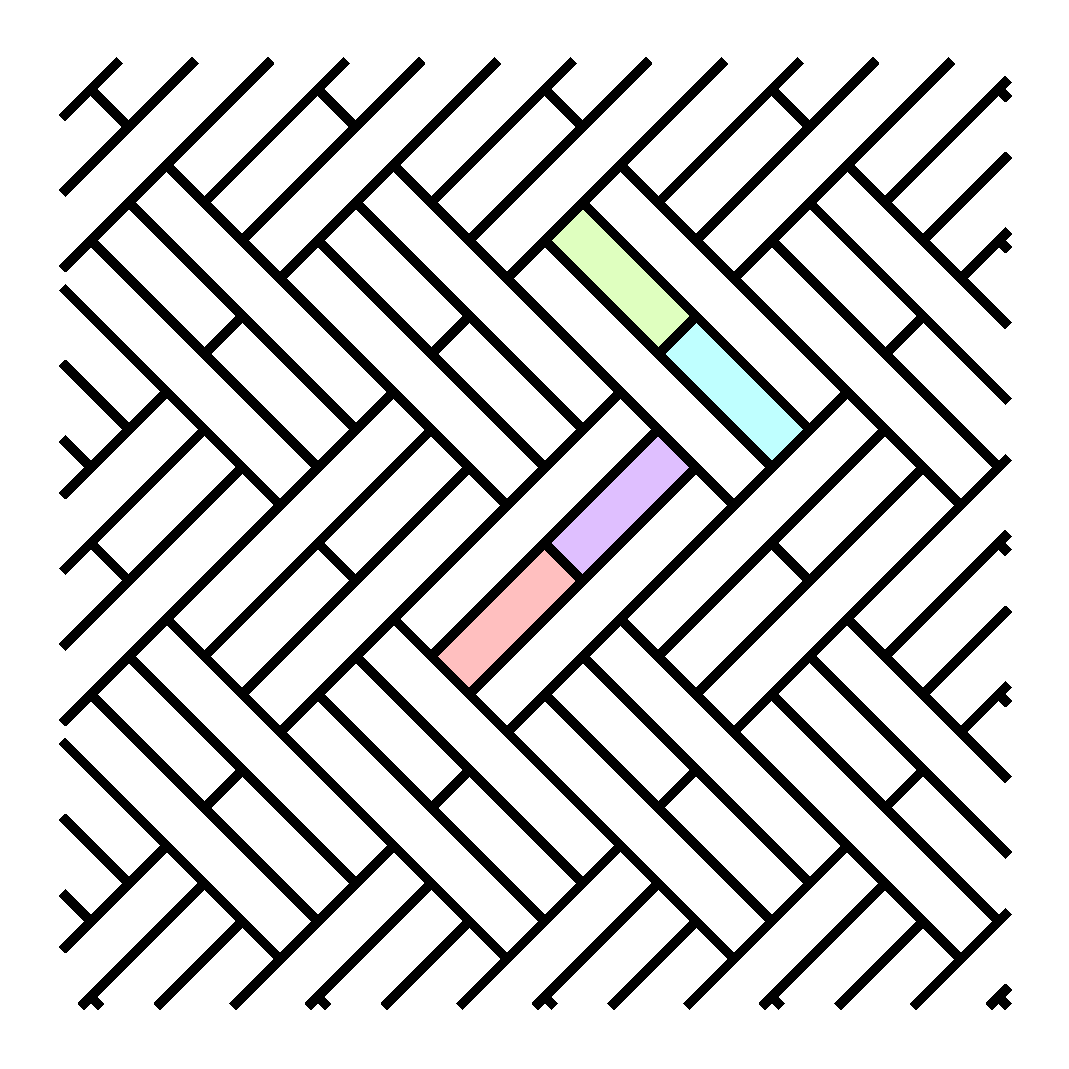
\includegraphics[width=1.9in]{c12}
  \end{center}
\end{frame}

\begin{frame}
  \begin{center}
    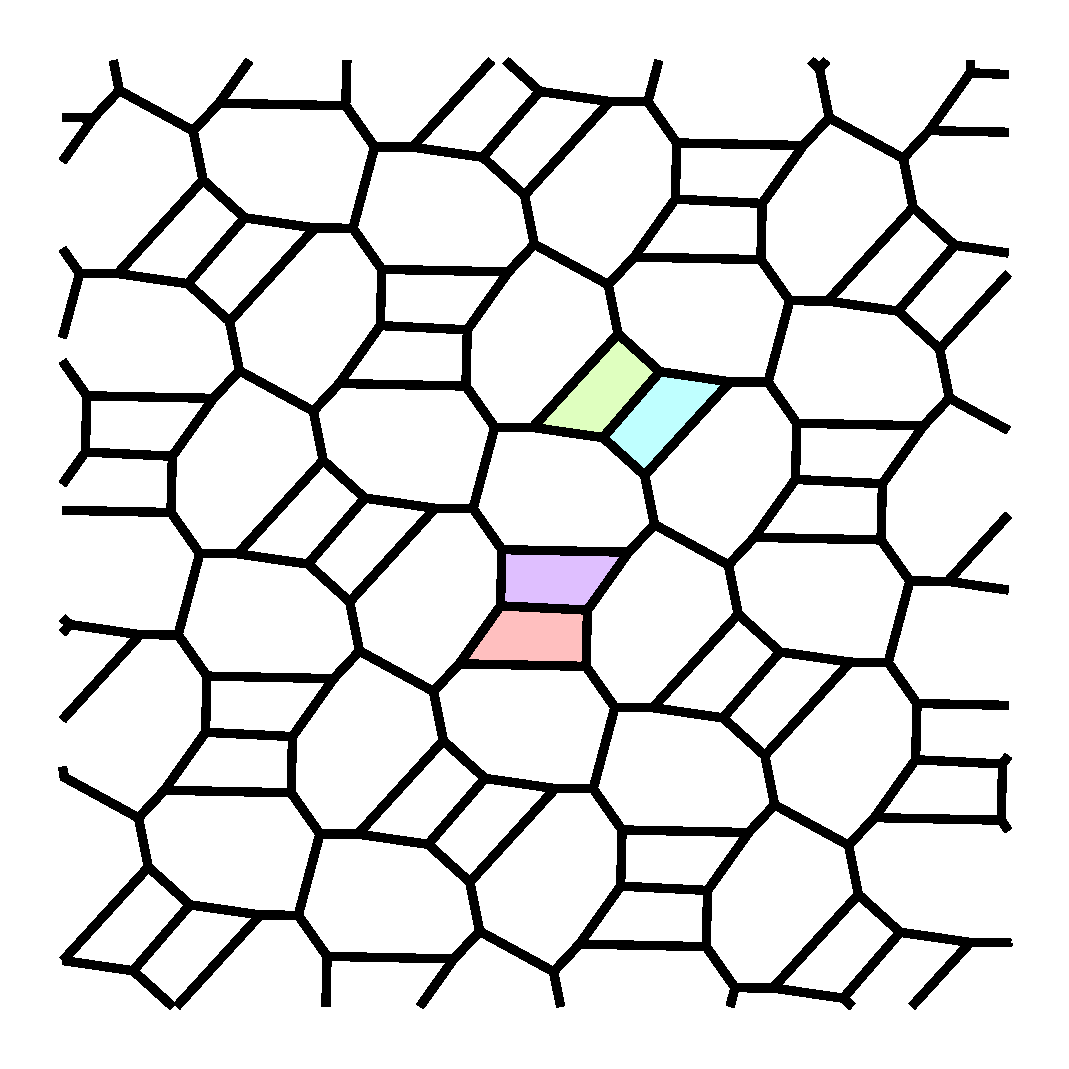
\includegraphics[width=1.9in]{c08}
    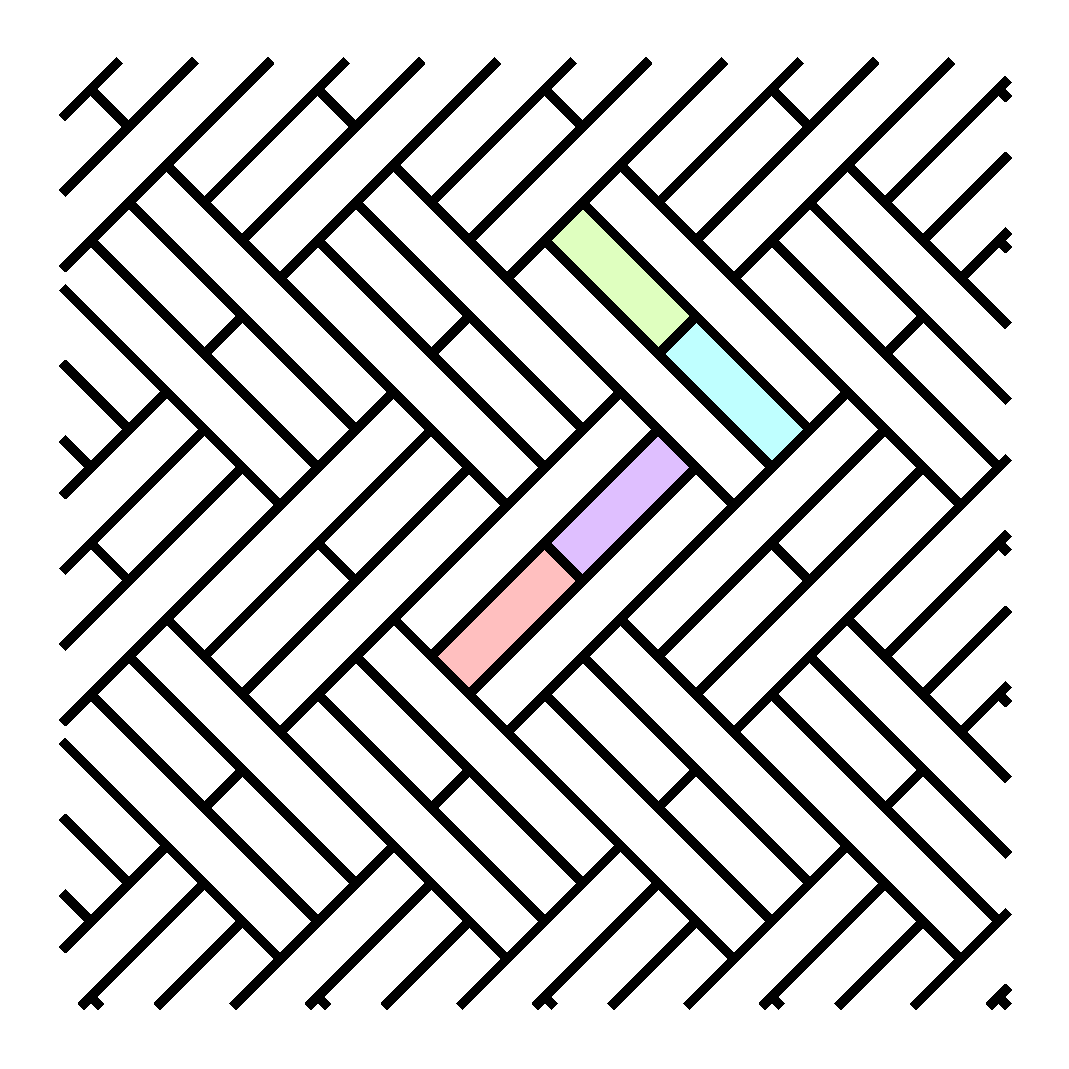
\includegraphics[width=1.9in]{c12}
  \end{center}
\end{frame}

\begin{frame}
  \begin{center}
    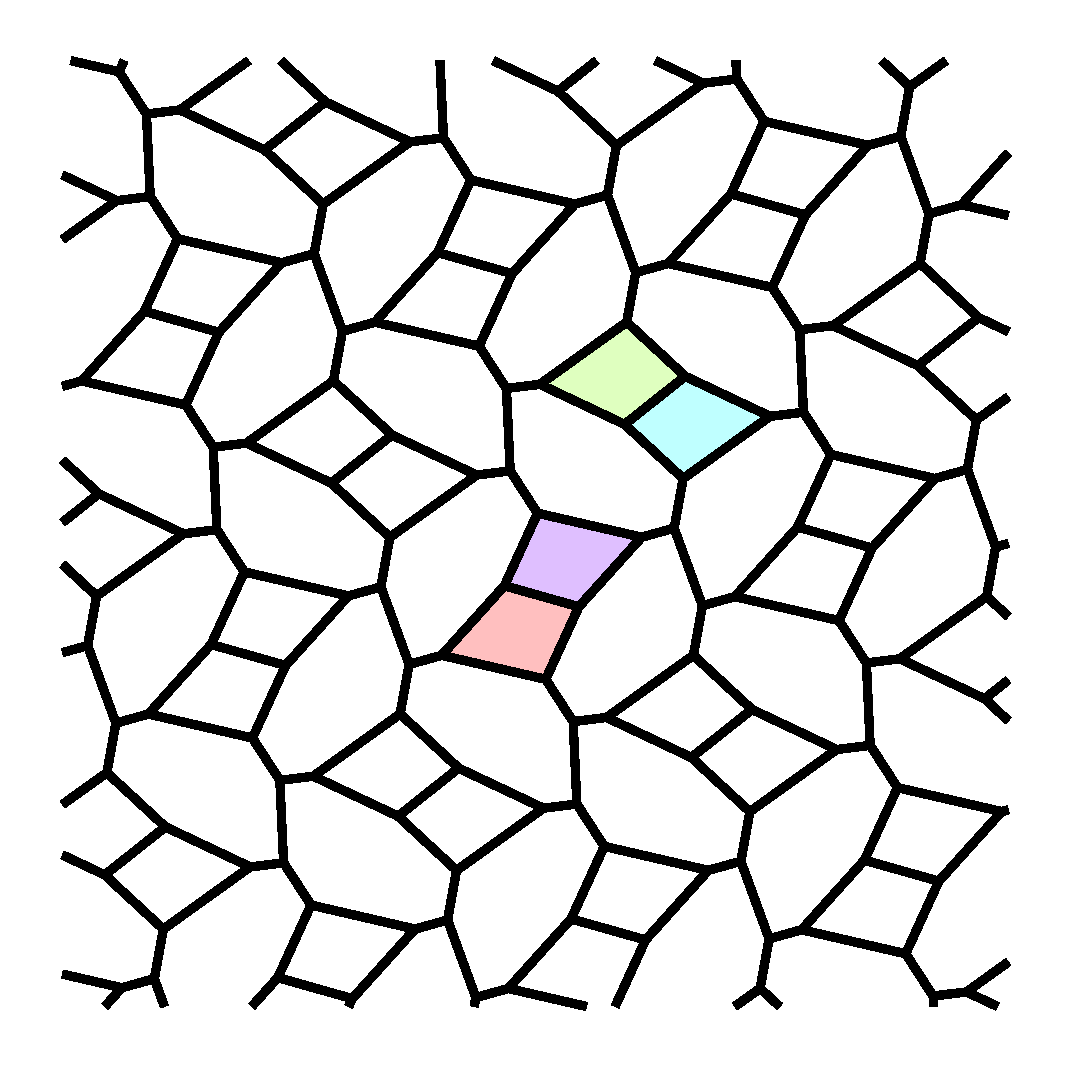
\includegraphics[width=1.9in]{c09}
    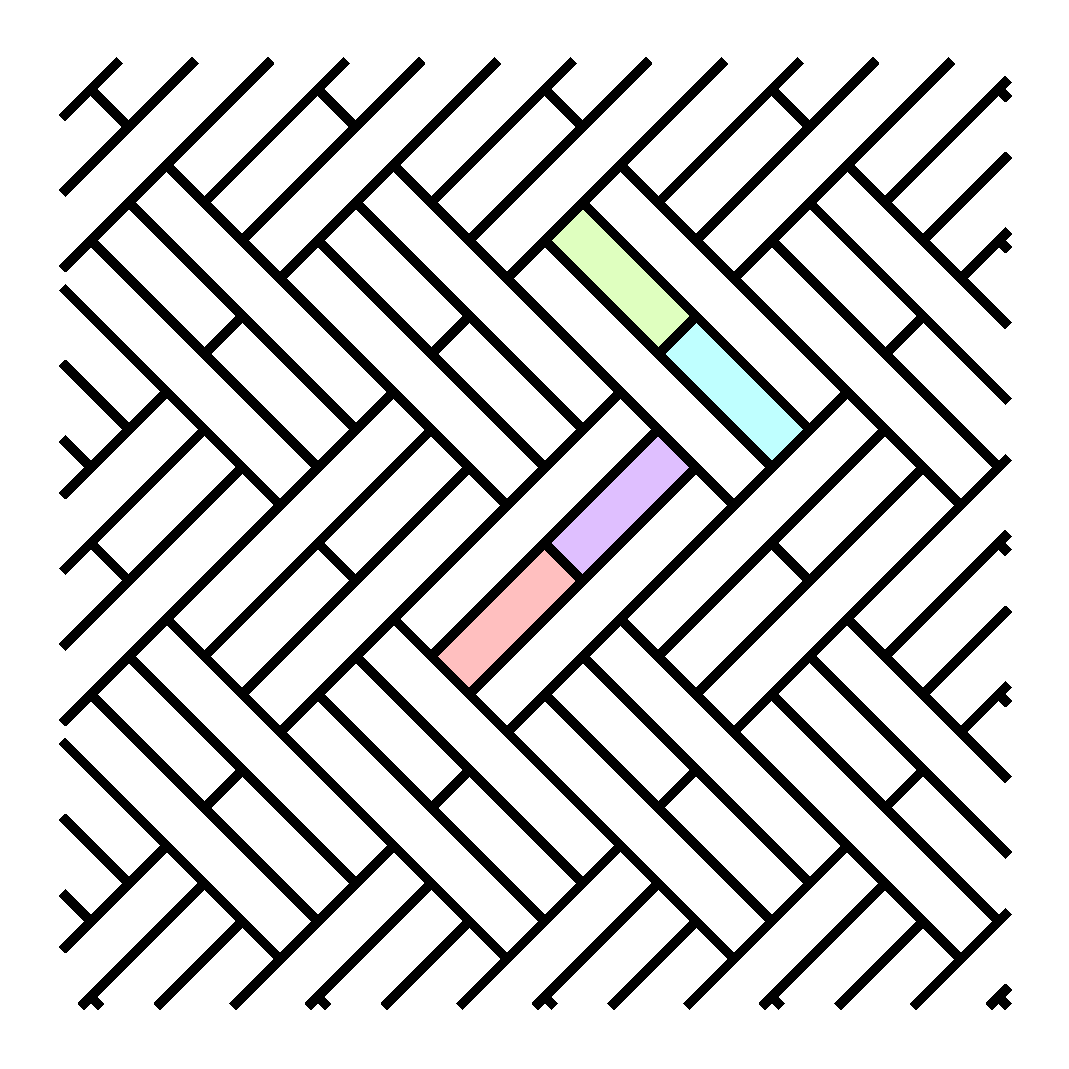
\includegraphics[width=1.9in]{c12}
  \end{center}
\end{frame}

\begin{frame}
  \begin{center}
    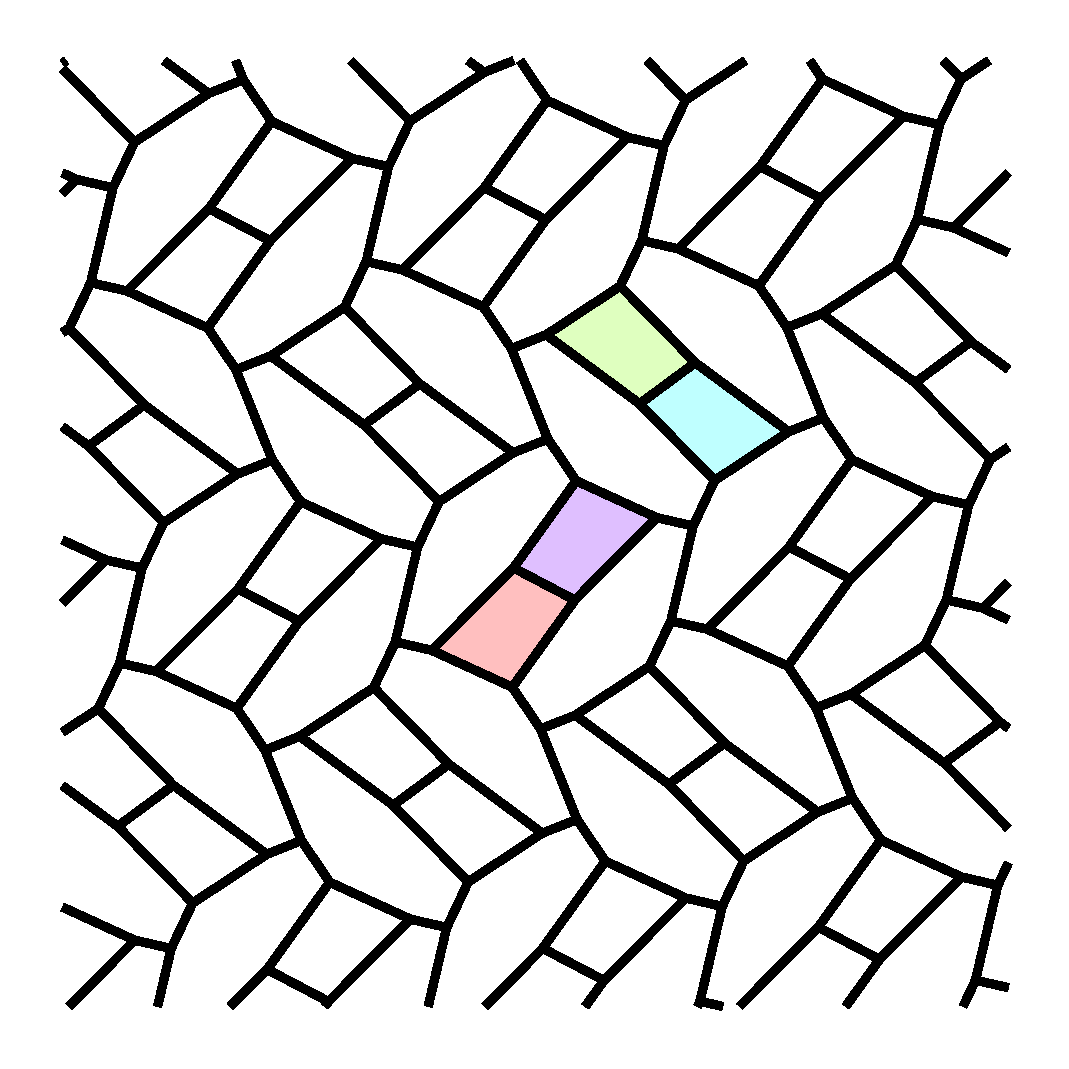
\includegraphics[width=1.9in]{c10}
    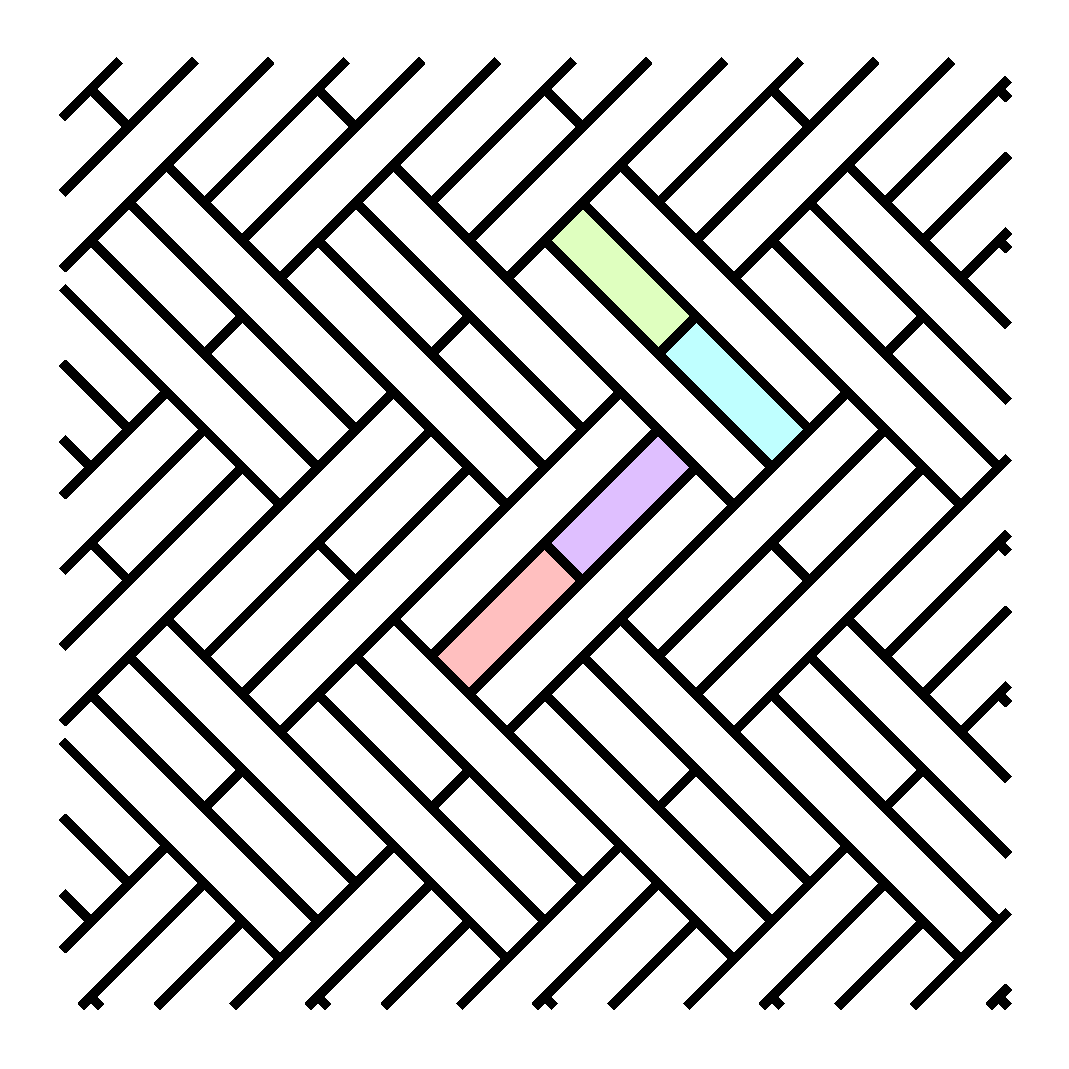
\includegraphics[width=1.9in]{c12}
  \end{center}
\end{frame}

\begin{frame}
  \begin{center}
    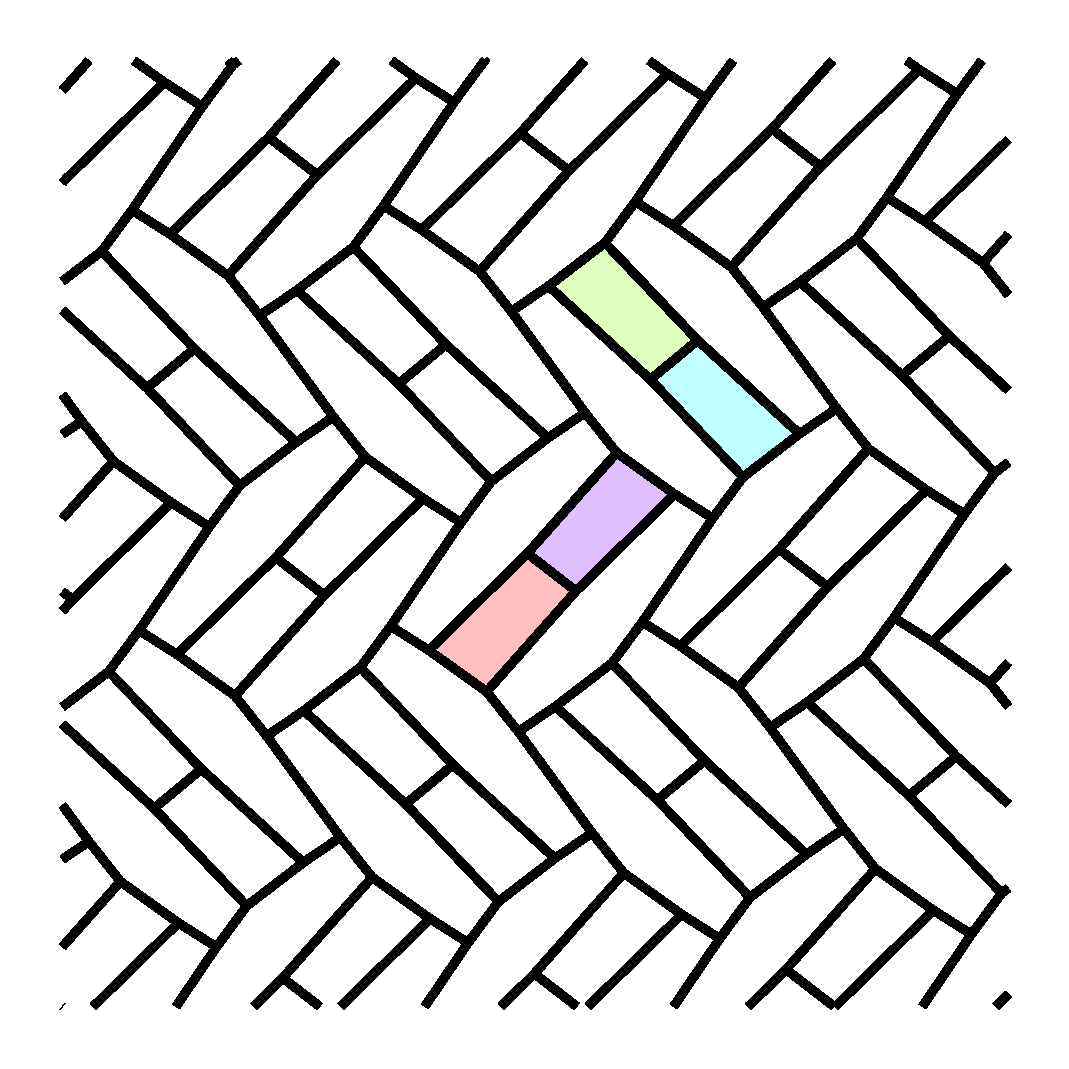
\includegraphics[width=1.9in]{c11}
    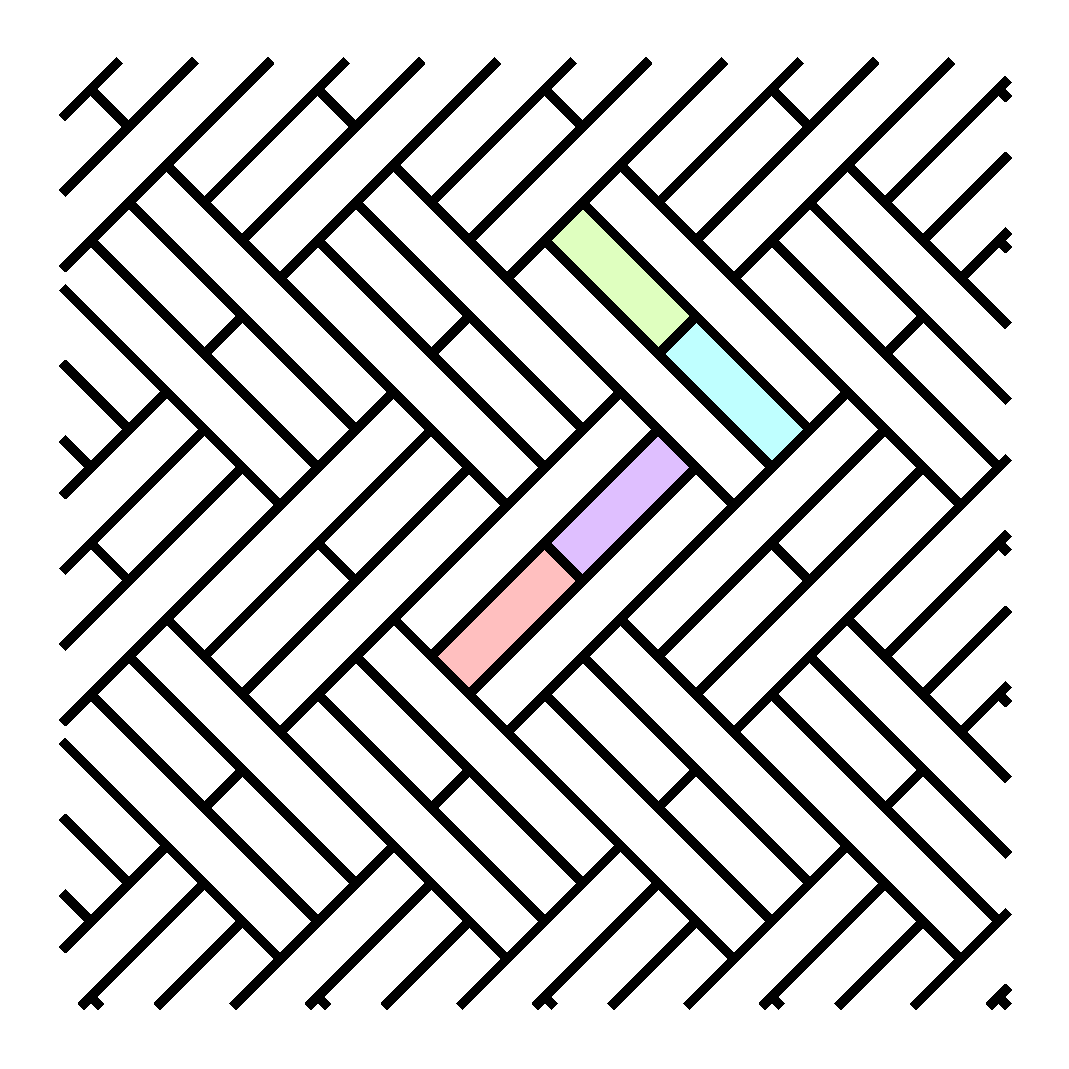
\includegraphics[width=1.9in]{c12}
  \end{center}
\end{frame}

\begin{frame}
  \begin{center}
    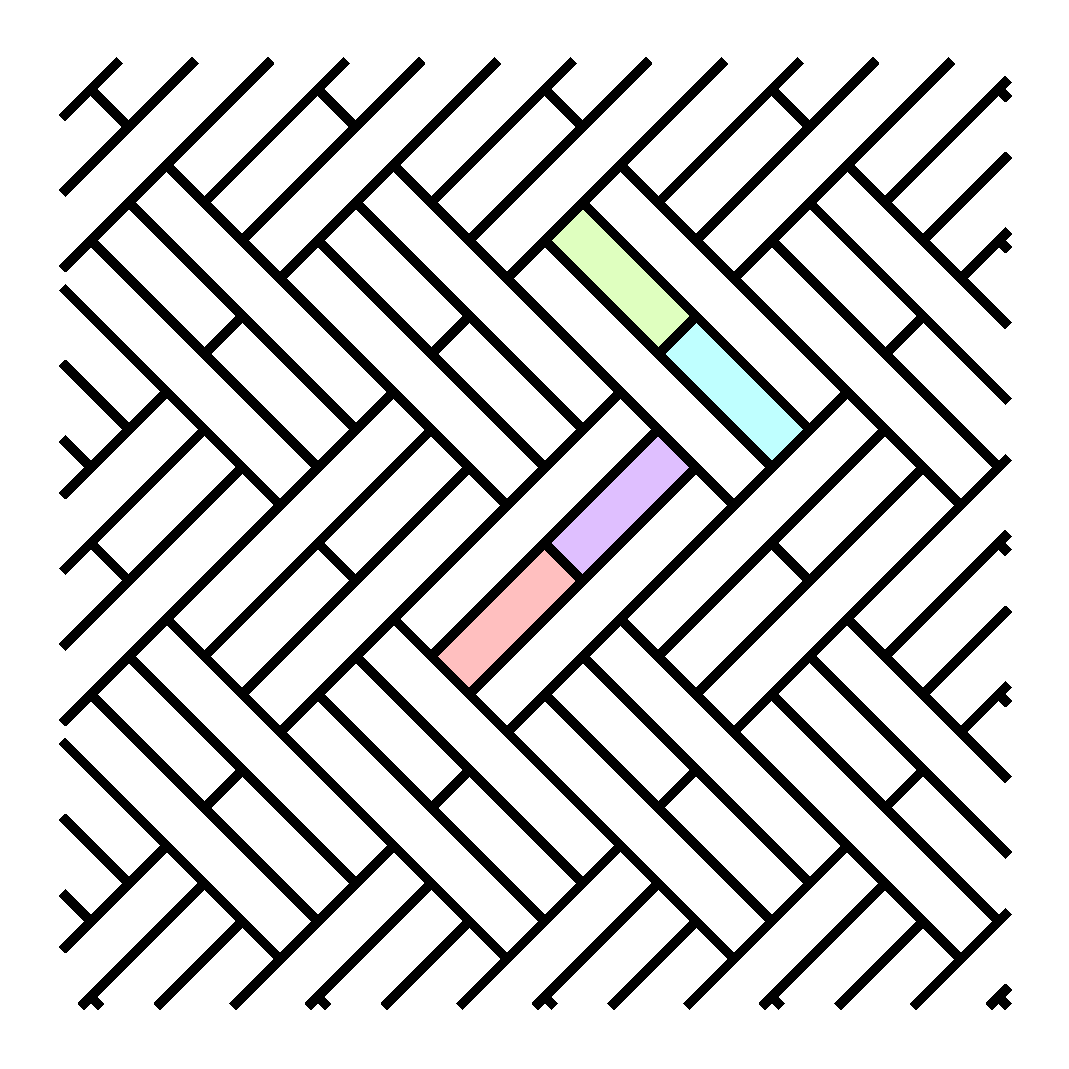
\includegraphics[width=1.9in]{c12}
    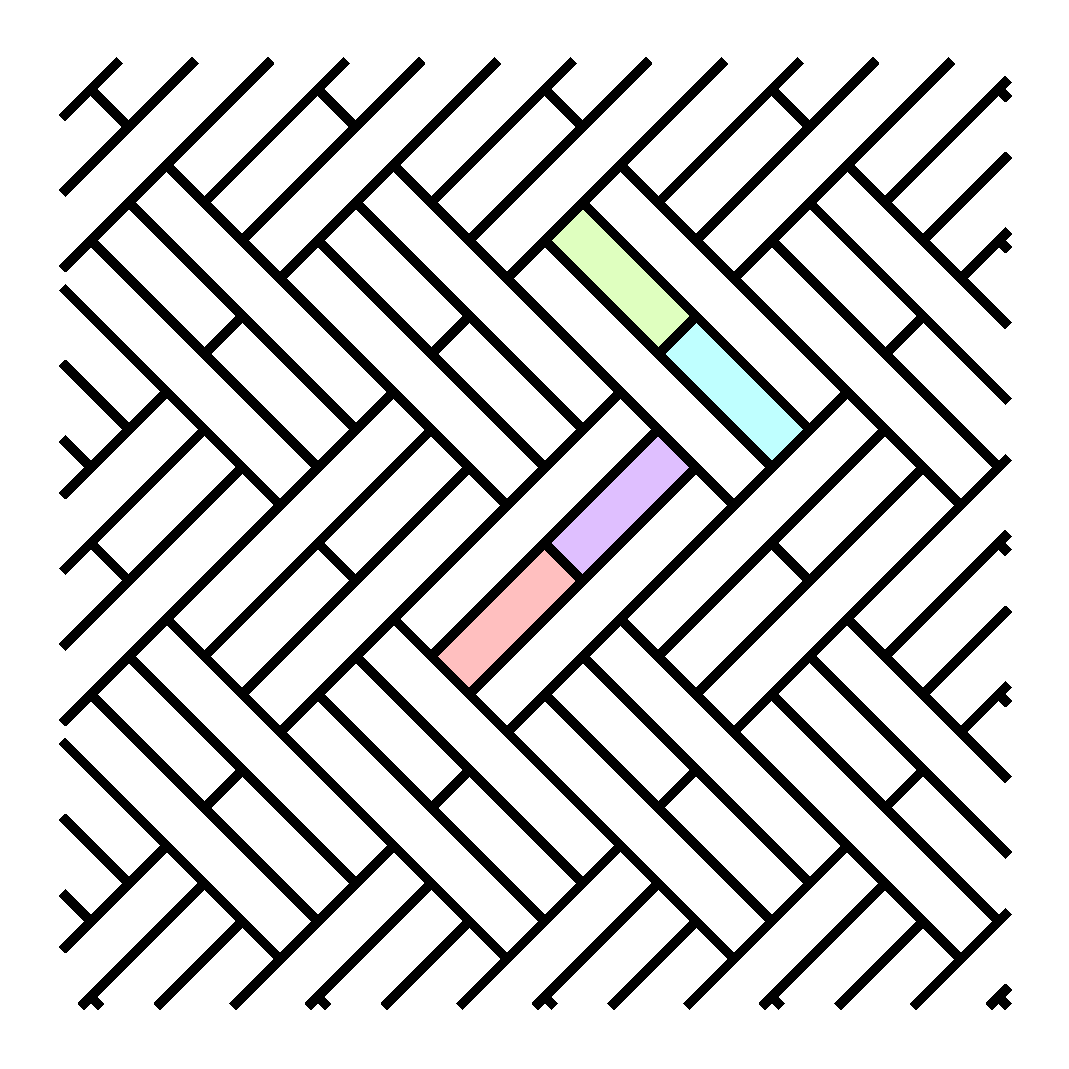
\includegraphics[width=1.9in]{c12}
  \end{center}
\end{frame}


\section{Delaney-Dress Symbols}

\begin{frame}
  \begin{center}
    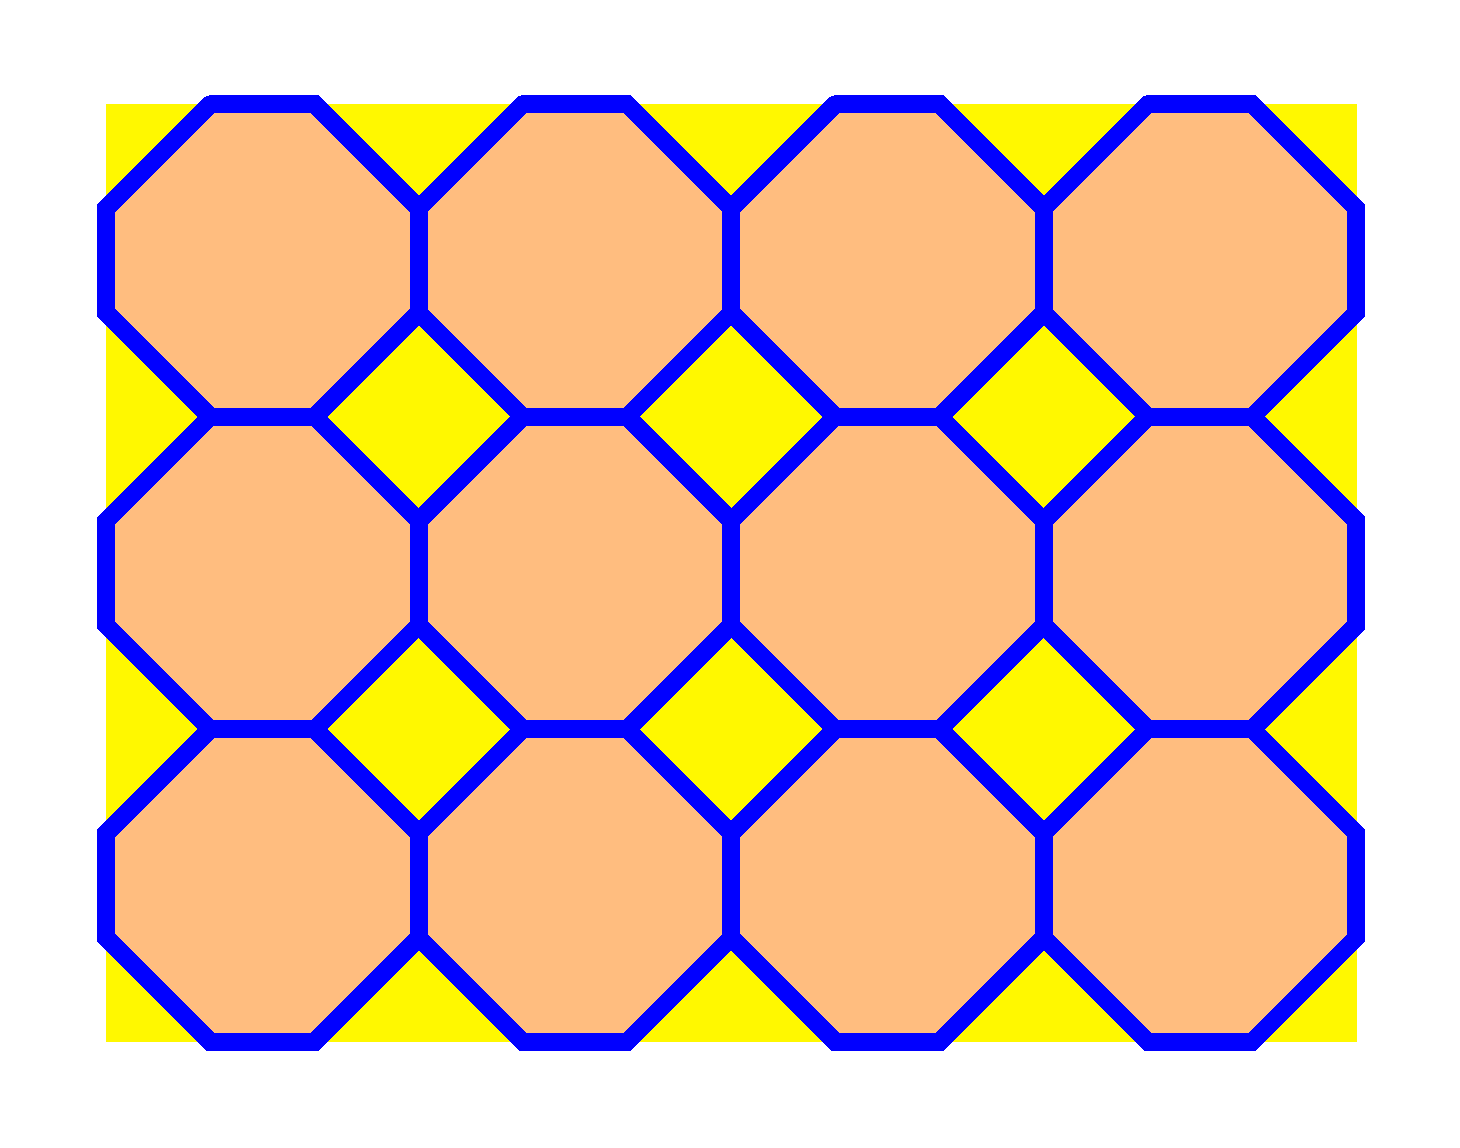
\includegraphics[width=3.5in]{dsymbol1}
  \end{center}
\end{frame}

\begin{frame}
  \begin{center}
    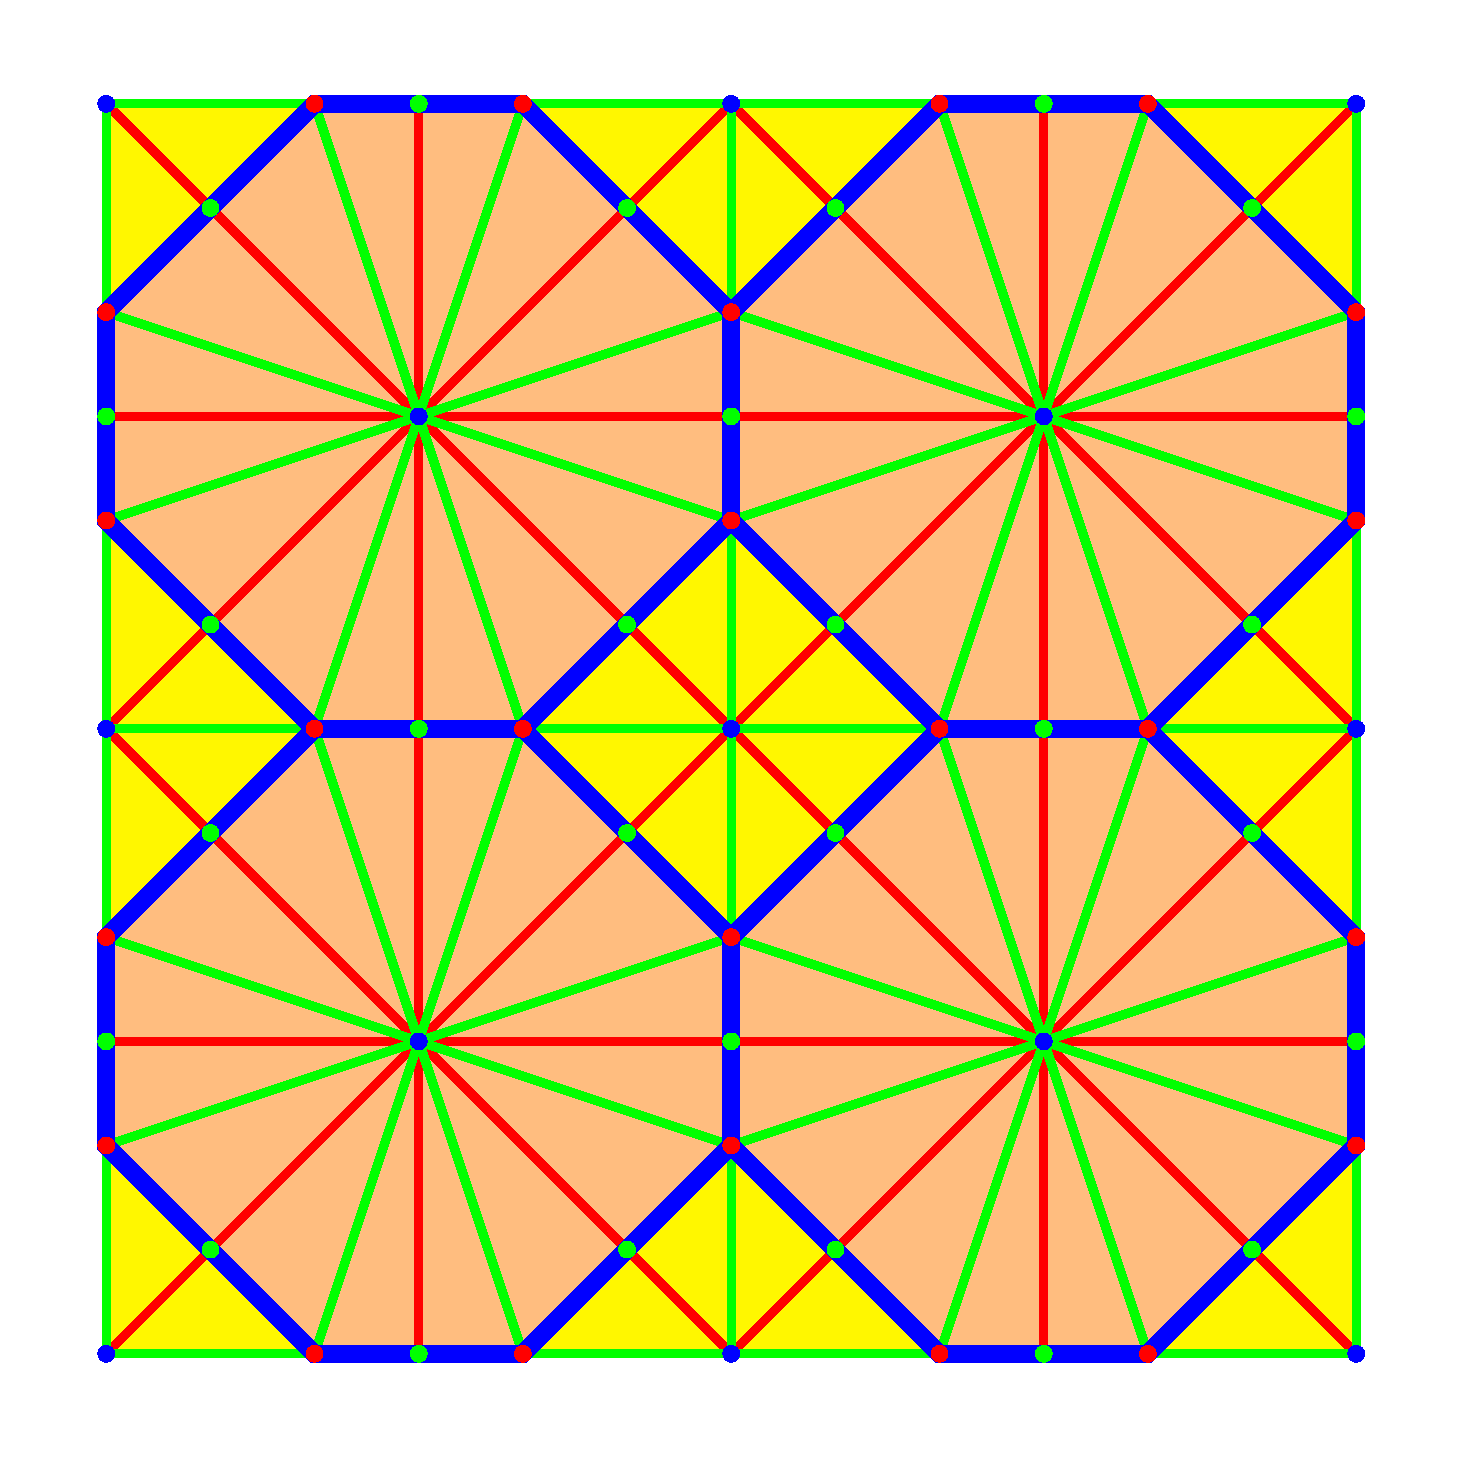
\includegraphics[width=3.5in]{dsymbol2}
  \end{center}
\end{frame}

\begin{frame}
  \begin{center}
    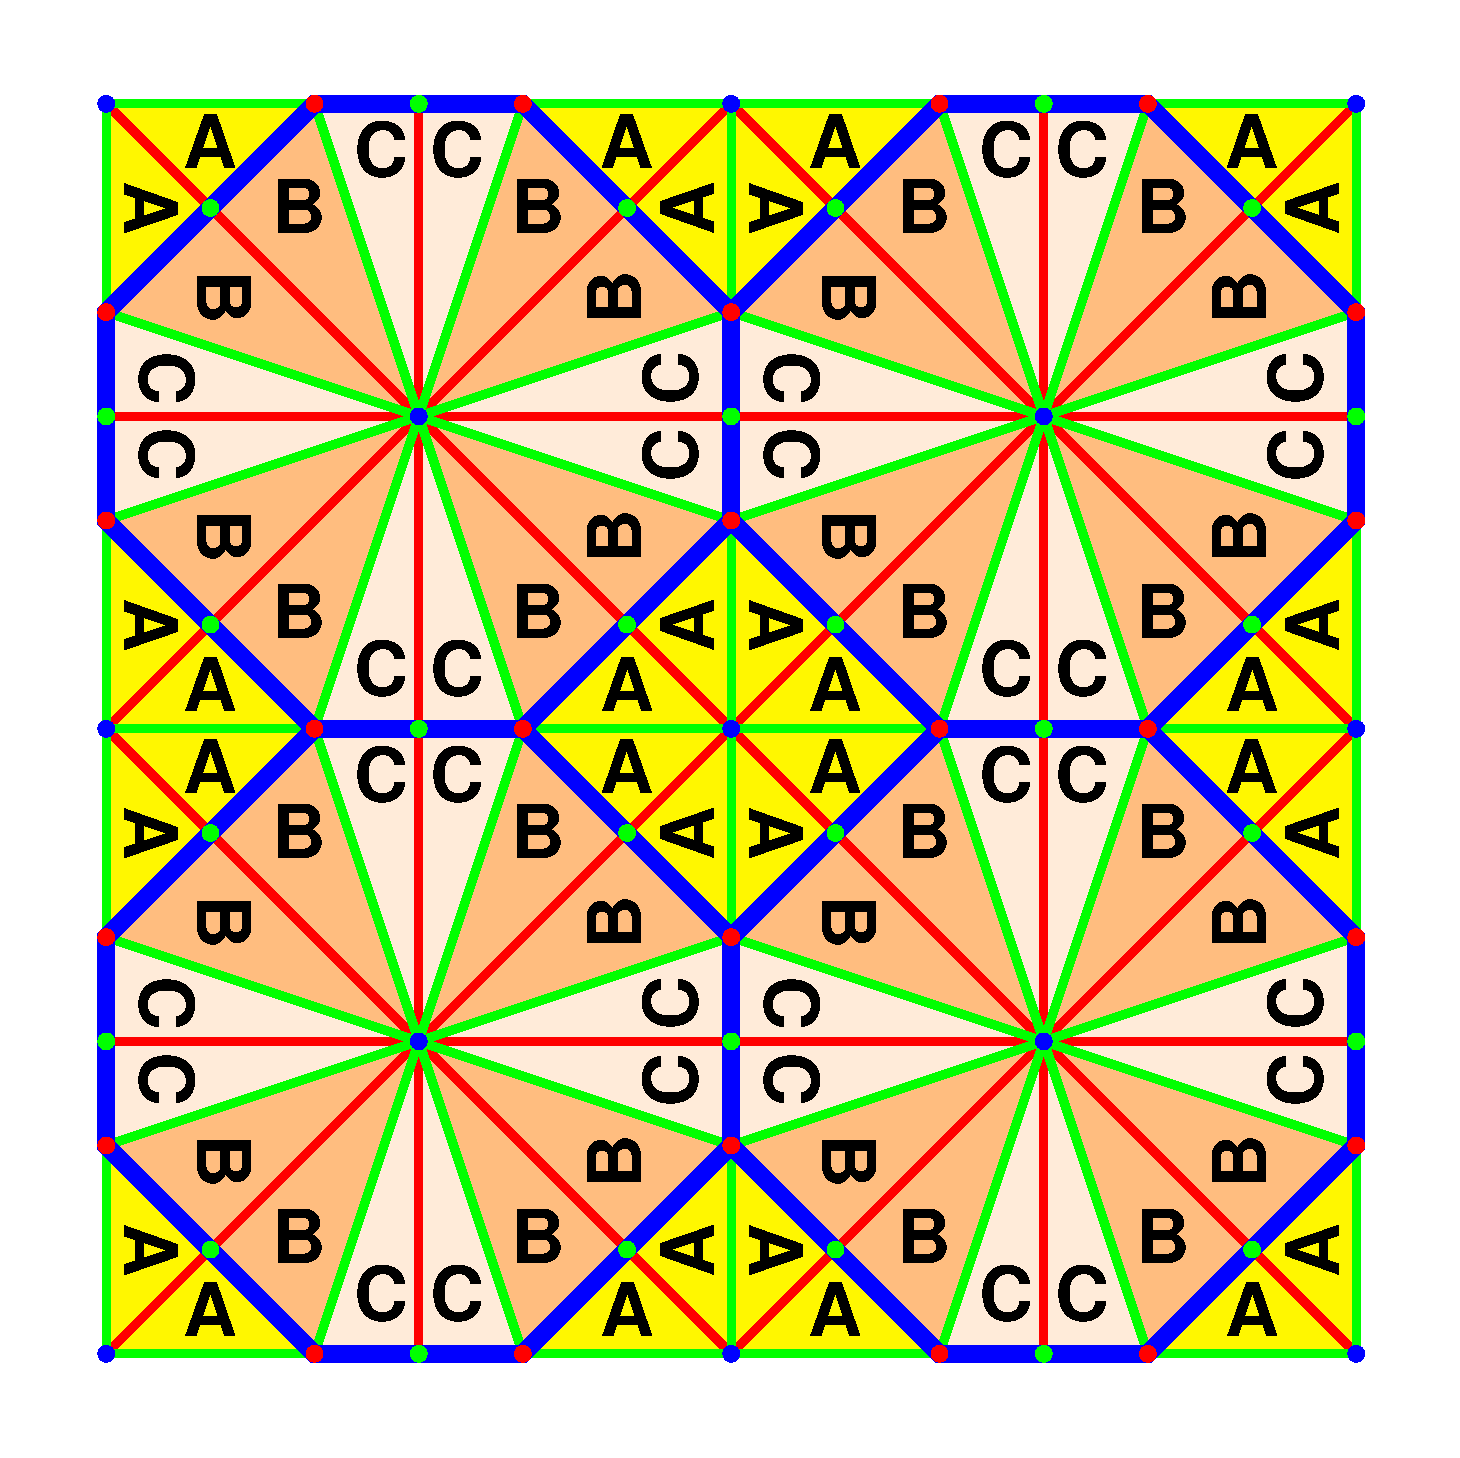
\includegraphics[width=1.9in]{dsymbol3}
    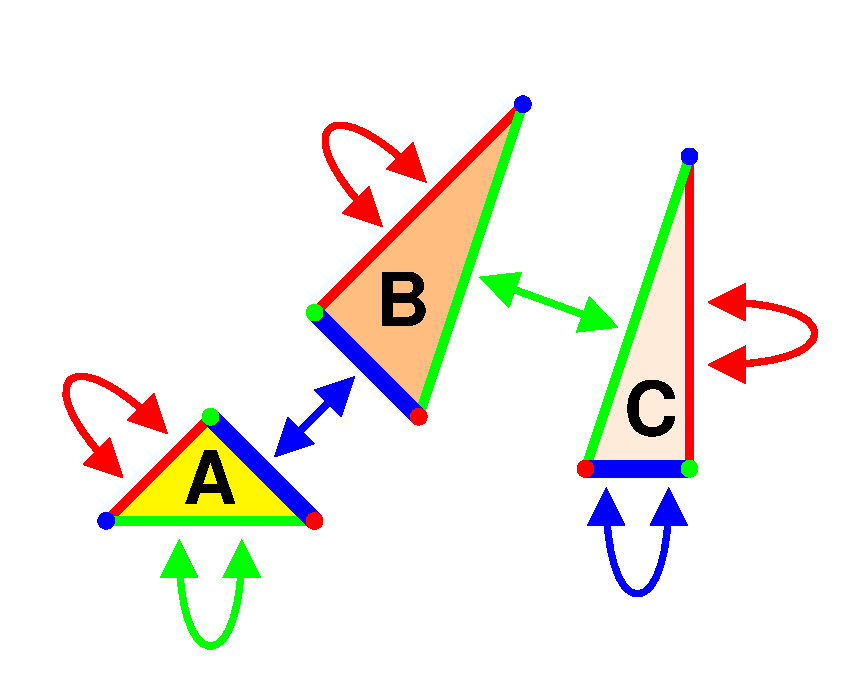
\includegraphics[width=1.9in]{dsymbol4}
  \end{center}
\end{frame}

\begin{frame}
  \begin{center}
    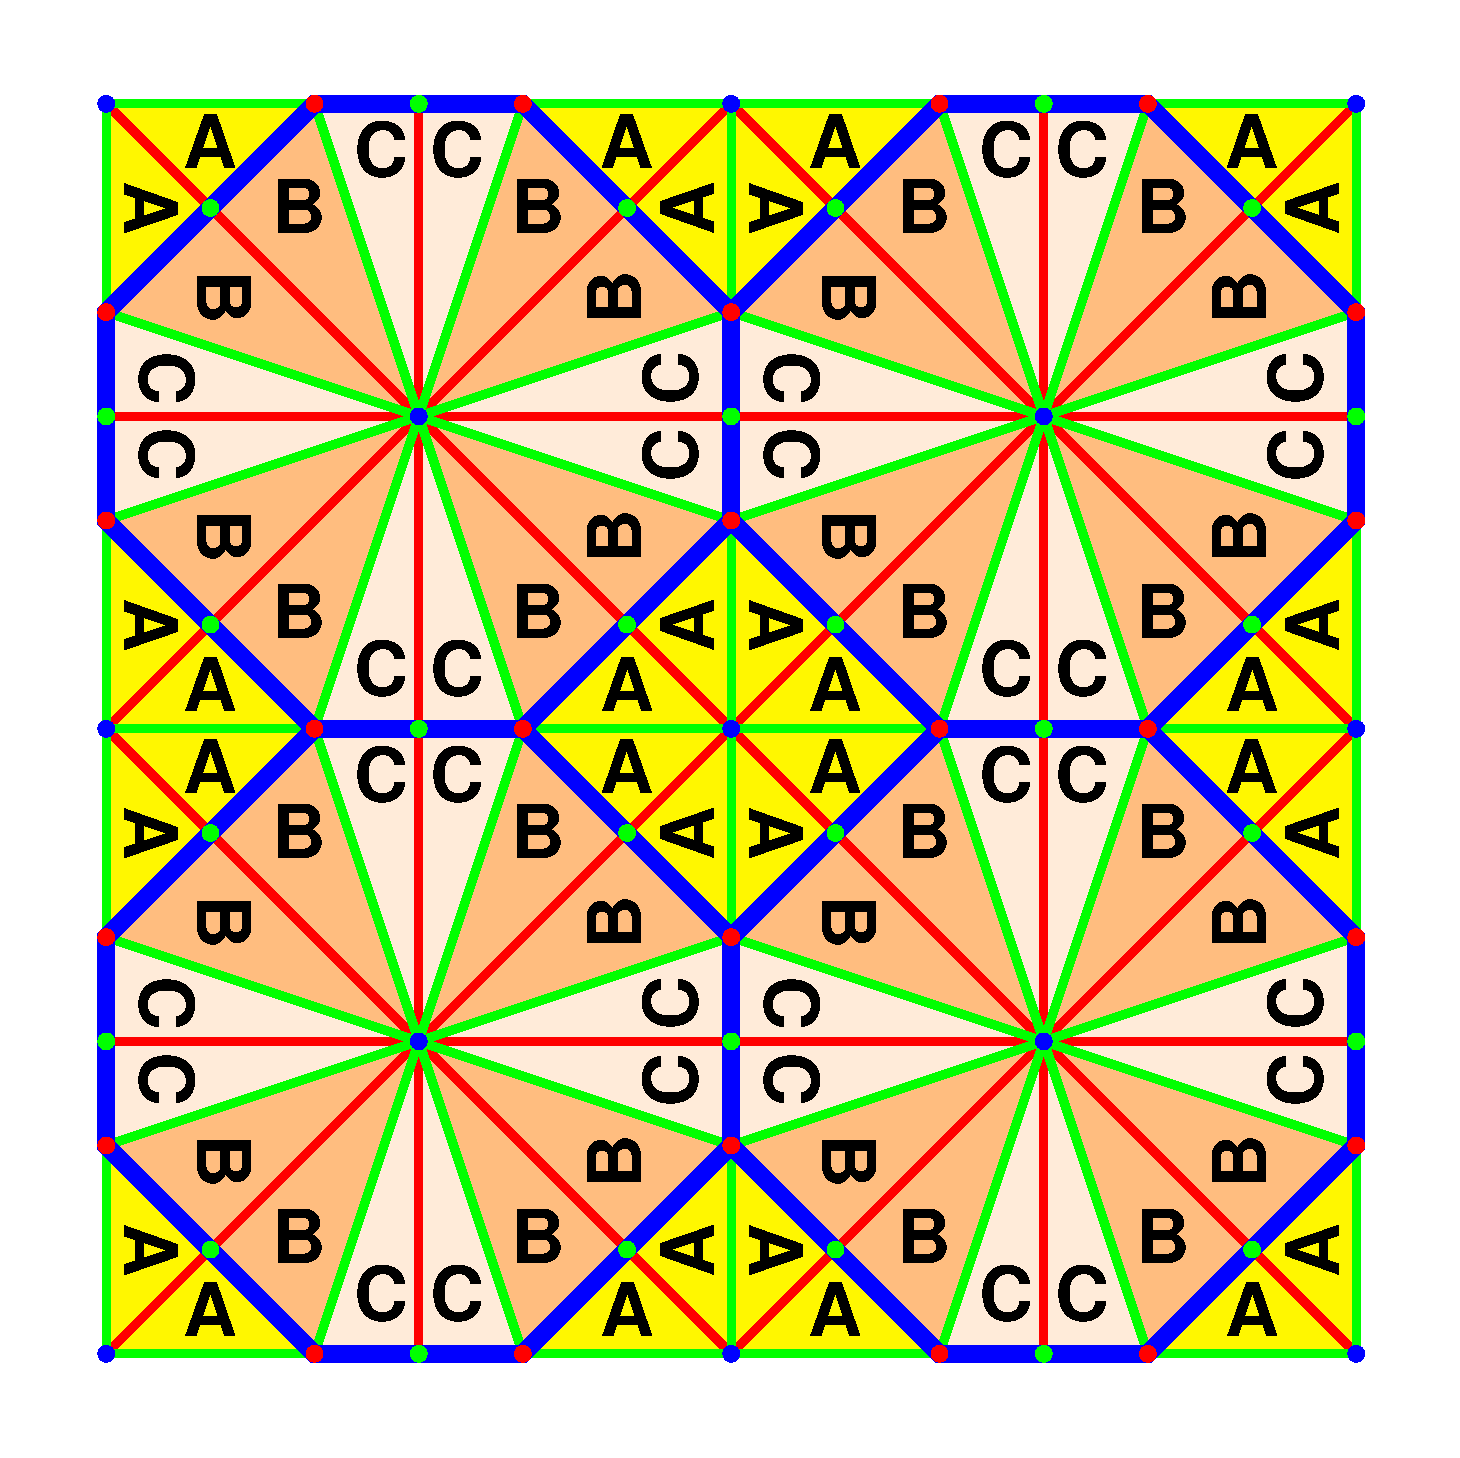
\includegraphics[width=1.9in]{dsymbol3}
    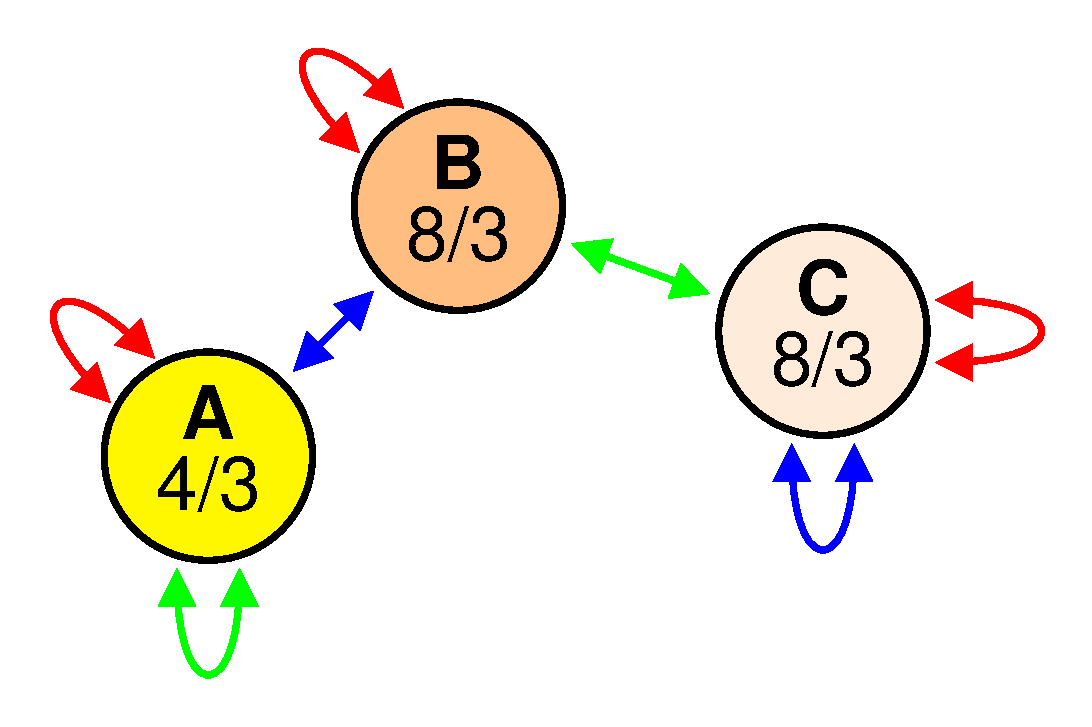
\includegraphics[width=1.9in]{dsymbol5}
  \end{center}
\end{frame}


\section{Heaven And Hell}

\begin{frame}
  \begin{center}
    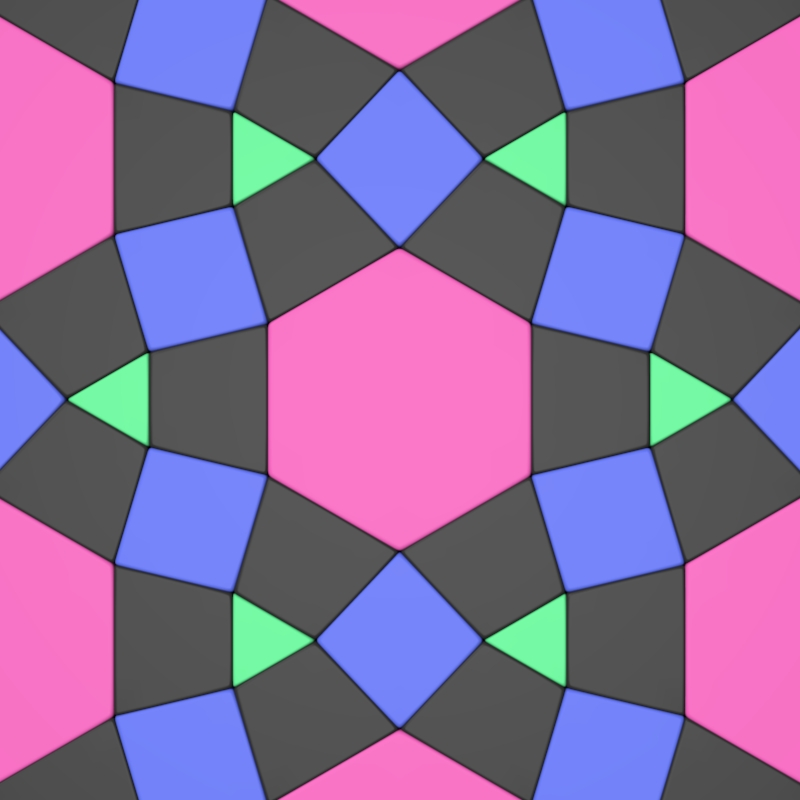
\includegraphics[width=3.5in]{hh13}
  \end{center}
\end{frame}

\begin{frame}
  \includegraphics[width=0.6in]{hh01}
  \hspace{0.1mm}
  \includegraphics[width=0.6in]{hh02}
  \hspace{0.1mm}
  \includegraphics[width=0.6in]{hh03}
  \hspace{0.1mm}
  \includegraphics[width=0.6in]{hh04}
  \hspace{0.1mm}
  \includegraphics[width=0.6in]{hh05}
  \hspace{0.1mm}
  \includegraphics[width=0.6in]{hh06}\\[0.7mm]

  \includegraphics[width=0.6in]{hh07}
  \hspace{0.1mm}
  \includegraphics[width=0.6in]{hh08}
  \hspace{0.1mm}
  \includegraphics[width=0.6in]{hh09}
  \hspace{0.1mm}
  \includegraphics[width=0.6in]{hh10}
  \hspace{0.1mm}
  \includegraphics[width=0.6in]{hh11}
  \hspace{0.1mm}
  \includegraphics[width=0.6in]{hh12}\\[0.7mm]

  \includegraphics[width=0.6in]{hh13}
  \hspace{0.1mm}
  \includegraphics[width=0.6in]{hh14}
  \hspace{0.1mm}
  \includegraphics[width=0.6in]{hh15}
  \hspace{0.1mm}
  \includegraphics[width=0.6in]{hh16}
  \hspace{0.1mm}
  \includegraphics[width=0.6in]{hh17}
  \hspace{0.1mm}
  \includegraphics[width=0.6in]{hh18}\\[0.7mm]

  \includegraphics[width=0.6in]{hh19}
  \hspace{0.1mm}
  \includegraphics[width=0.6in]{hh20}
  \hspace{0.1mm}
  \includegraphics[width=0.6in]{hh21}
  \hspace{0.1mm}
  \includegraphics[width=0.6in]{hh22}
  \hspace{0.1mm}
  \includegraphics[width=0.6in]{hh23}

  \begin{center}
    {\small
      A.W.M.\ Dress, D.H.\ Huson. {\it Revue Topologie Structurale}, 1991
    }
  \end{center}
\end{frame}


\section{3d Tilings And Materials}

\begin{frame}
  \begin{center}
    \includegraphics[width=3.5in]{cube-barycentric}
  \end{center}
\end{frame}

\begin{frame}
  \begin{center}
    \includegraphics[width=3.5in]{platonic}\\[1cm]
    \includegraphics[height=1.2in]{diamond-fill}
    \hspace{1cm}
    \includegraphics[height=1.2in]{diamond-voronoi}
  \end{center}
\end{frame}


\section{Simple Tilings}

\begin{frame}
  \begin{center}
    \includegraphics[width=3.5in]{simple8}
  \end{center}
\end{frame}

\begin{frame}
  \begin{center}
    \includegraphics[width=1.0in]{simple1}
    \includegraphics[width=1.0in]{simple2}
    \includegraphics[width=1.0in]{simple3}\\
    \includegraphics[width=1.0in]{simple4}
    \includegraphics[width=1.0in]{simple5}
    \includegraphics[width=1.0in]{simple6}\\
    \includegraphics[width=1.0in]{simple7}
    \includegraphics[width=1.0in]{simple8}
    \includegraphics[width=1.0in]{simple9}
  \end{center}
\end{frame}


\section{Is Diamond Simple}

\begin{frame}
  \begin{center}
    \includegraphics[height=1.0in]{extetra1}
    \hspace{2mm}
    \includegraphics[height=1.0in]{extetra2}
    \hspace{2mm}
    \includegraphics[height=1.0in]{extetra3}\\[2mm]
    \includegraphics[height=2.0in]{diamond-tiling}
  \end{center}
\end{frame}


\section{Demo}

\begin{frame}
  \begin{center}
    Demo
  \end{center}
\end{frame}

\end{document}
